\documentclass[output=paper,hidelinks]{langscibook}
\ChapterDOI{10.5281/zenodo.10185970}
\title{Prosody and its interfaces}
\author{Tina Bögel\affiliation{University of Konstanz}}
\abstract{LFG has always had a strong focus on syntax and semantics, but the last two decades have seen significant progress with regard to the integration of p(ho\-nol\-o\-gical)-structure into LFG. This chapter first briefly introduces important concepts for the analysis of prosody and gives an overview of widely adopted approaches to the syntax--prosody interface. The second part surveys the different proposals for the integration of  p-structure and its interfaces into LFG, with a particular focus on the architectural assumptions behind each approach and the resulting implications for the architecture of grammar.}

\IfFileExists{../localcommands.tex}{
   \addbibresource{../localbibliography.bib}
   \addbibresource{thisvolume.bib}
   \usepackage{langsci-optional}
\usepackage{langsci-gb4e}
\usepackage{langsci-lgr}

\usepackage{listings}
\lstset{basicstyle=\ttfamily,tabsize=2,breaklines=true}

%added by author
% \usepackage{tipa}
\usepackage{multirow}
\graphicspath{{figures/}}
\usepackage{langsci-branding}

   
\newcommand{\sent}{\enumsentence}
\newcommand{\sents}{\eenumsentence}
\let\citeasnoun\citet

\renewcommand{\lsCoverTitleFont}[1]{\sffamily\addfontfeatures{Scale=MatchUppercase}\fontsize{44pt}{16mm}\selectfont #1}
  
   %% hyphenation points for line breaks
%% Normally, automatic hyphenation in LaTeX is very good
%% If a word is mis-hyphenated, add it to this file
%%
%% add information to TeX file before \begin{document} with:
%% %% hyphenation points for line breaks
%% Normally, automatic hyphenation in LaTeX is very good
%% If a word is mis-hyphenated, add it to this file
%%
%% add information to TeX file before \begin{document} with:
%% %% hyphenation points for line breaks
%% Normally, automatic hyphenation in LaTeX is very good
%% If a word is mis-hyphenated, add it to this file
%%
%% add information to TeX file before \begin{document} with:
%% \include{localhyphenation}
\hyphenation{
affri-ca-te
affri-ca-tes
an-no-tated
com-ple-ments
com-po-si-tio-na-li-ty
non-com-po-si-tio-na-li-ty
Gon-zá-lez
out-side
Ri-chárd
se-man-tics
STREU-SLE
Tie-de-mann
}
\hyphenation{
affri-ca-te
affri-ca-tes
an-no-tated
com-ple-ments
com-po-si-tio-na-li-ty
non-com-po-si-tio-na-li-ty
Gon-zá-lez
out-side
Ri-chárd
se-man-tics
STREU-SLE
Tie-de-mann
}
\hyphenation{
affri-ca-te
affri-ca-tes
an-no-tated
com-ple-ments
com-po-si-tio-na-li-ty
non-com-po-si-tio-na-li-ty
Gon-zá-lez
out-side
Ri-chárd
se-man-tics
STREU-SLE
Tie-de-mann
}
   \togglepaper[17]%%chapternumber
}{}

\begin{document}
\maketitle
\label{chap:Prosody}

\section{Introduction}

LFG has always had a strong focus on syntax and semantics. However, with the realisation that prosodic information can significantly contribute to linguistic analyses and is often crucial for the correct interpretation of meaning (e.g., in form of prosodic disambiguation of syntactically ambiguous structures or for the correct interpretation of information structure), the last two decades have seen significant progress with regard to the integration of prosodic structure into LFG. 

LFG assumes that different aspects of grammar (i.e., syntax, semantics, etc.) are represented by unique modules (also called `projections'), each guided by its own principles and constraints, and with representations well-suited to their unique functions  (cf.~\citealt{dalrymple01, Sadock91}, see also \citetv{chapters/Intro}).
The syntactic component, for example, is represented by c(onstituent)- and f(unctional)-structure and is concerned with constituency (via phrase structure rules) and the encoding of grammatical functions and morphosyntactic features, while phonology (including prosody) is represented by p(honological)-structure and is concerned with phonological and prosodic properties like pro\-sod\-ic phrasing, rhythmic constraints, and intonation.\footnote{In most of the approaches discussed in \sectref{sec:ps_LFG} the `p' in p-structure represents p(rosodic)-structure, as prosodic features ususally contain relevant information for analyses at the interfaces  to syntax, semantics, and information structure. However, prosody is only one part of the larger field of phonology and some phenomena that are not part of prosody (e.g., postlexical sandhi phenomena) can be closely interlaced with prosody in that they can indicate a specific prosodic domain. This chapter will thus use the term p(honological)-structure, of which prosody is part, but which does not, per se, restrict p-structure to represent prosody alone. }

Communication between the different modules is handled by LFG's correspondence architecture, which allows for relevant information to be made available at the respective interfaces. The establishment of these interfaces necessarily presumes a specific grammar architecture; that is, it presupposes an explicit positioning of modules with respect to each other. 
Discussing the architectural assumptions made in each p-structure proposal is thus essential for the understanding of the (in parts fundamental) differences in the representation of prosody and the communication at the interfaces.
 

This chapter provides an overview of the different approaches to prosody and its interfaces in LFG, and places these with respect to proposals made in the wider literature. It furthermore discusses the architectural assumptions made in each proposal and offers insights into a more general view of grammar. The chapter is structured as follows: \sectref{sec:pros_interfaces} provides a general introduction into two major aspects of prosody (phrasing and intonation)  and discusses current approaches to prosody and its interfaces in the wider literature. A discussion of the LFG grammar architecture and the placement of the phonological module (including prosody) is provided in \sectref{sec:Prosody:arch}. This section also establishes a fundamental difference between the proposals with respect to how grammar is viewed in general. \sectref{sec:ps_LFG} provides 
 a chronological overview of the different approaches to prosody and its interfaces in LFG, in particular with respect to the architectural assumptions made in each proposal. \sectref{sec:Conclusion} concludes the chapter.

%%%%%%%%%%%%%%%%%%%%%%%%%%%%%%%%%%%%%%%%%%%%%%%%%%%%%%%%%%%%%%
%%%%%%%%%%%%%%%%%%%%%%%%%%%%%%%%%%%%%%%%%%%%%%%%%%%%%%%%%%%%%%
%%%%%%%%%%%%%%%%%%%%%%%%%%%%%%%%%%%%%%%%%%%%%%%%%%%%%%%%%%%%%%

\section{Prosody and its interfaces}
\label{sec:pros_interfaces}
The LFG approaches to prosody discussed in \sectref{sec:ps_LFG} draw on a number of notions and theories established in the wider literature. This section first gives an overview on the general features that are particularly relevant with respect to the analysis of prosody at the interfaces and then describes the major approaches to the interface between syntax and prosody. 

%%%%%%%%%%%%%%%%%%%%%%%%%%%%%%%%%%%%%%%%%%%%%%%%%%%%%%%%%%%%%%
\subsection{What is prosody?}
\label{subsec:what_pros}
\noindent Prosody is a term used to describe suprasegmental phonology. It goes beyond the phonemic level of segmental phonology and is concerned with larger units in spoken language, including prosodic grouping, intonation and/or tones, rhythm, and stress patterns. Prosody can be used to express a number of properties and functions, among these clause type, clause structure, semantic scope, concepts of information structure such as topic and focus, but also speaker emotion, irony, or sarcasm. A detailed description of prosody goes far beyond the aim of this chapter and this section will only focus on some basic notions of prosody deemed fundamental for the current state of the art in LFG, namely prosodic phrasing, intonation, and the relationship between prosody and other modules of grammar.

Traditionally, it is assumed that spoken language is grouped into hierarchically structured {\bf prosodic domains} \citep[e.g.,][]{Selkirk1978, NesporVogel1986, Hayes1989}. 
Example (\ref{ex:pros_hier_1})  shows the most widely used proposal for the prosodic hierarchy originally  made in \citet{Selkirk1978} (building on an earlier proposal by \citealt{McCawley1968}; see also \citealt{Frota2012} for different suggestions).

\ea \label{ex:pros_hier_1} The Prosodic Hierarchy \citep{Selkirk1978}
{\small
\begin{center}
\begin{tabularx}{0.25\textwidth}{cl}
\multicolumn{2}{l}{\bf Prosodic hierarchy}\\[2ex]
\texttt{U} & utterance (Ut)\\
\textbar\\
$\iota$ & intonational phrase (IntP)\\
\textbar & \\
$\varphi$ & phonological phrase (PhP) \\
\textbar & \\
$\omega$ & prosodic word (PW)\\
\textbar & \\
{\tiny$\sum$} & foot (Ft)\\
\textbar & \\
$\sigma$ & syllable (Syll)
\end{tabularx}
\end{center}}
\z

In addition, the constraints in (\ref{ex:Prosody:2}) are assumed to apply to the prosodic hierarchy.\footnote{These constraints have been challenged and are now mostly considered to be `soft' constraints, see, e.g., \citet{BennettElfner2019}.}

\newpage
\ea \label{ex:Prosody:2}{\bf Constraints on Prosodic Domination \citep[ex.~4]{Selkirk1995}}\\
(where C$^n$ = some prosodic category)
\begin{itemize}
\item[(i)\ \ ] {\em Layeredness:} No C$^i$ dominates a C$^j$, j > i,\\
\indent\hspace{2ex} e.g.~``No syllable dominates a foot.''
\item[(ii)\ ] {\em Headedness:} Any C$^i$ must dominate a C$^{i-1}$ (except if C$^i$ = syllable),\\
\indent\hspace{2ex} e.g.~``A prosodic word must dominate a foot.''
\item[(iii)] {\em Exhaustivity:} No C$^i$ immediately dominates a constituent C$^j$, j < i-1,\\
\indent\hspace{2ex} e.g.~``No prosodic word immediately dominates a syllable.''
\item[(iv)] {\em Nonrecursivity:} No C$^i$ dominates C$^j$, j=i,\\
\indent\hspace{2ex} e.g.~``No foot dominates a foot.''
\end{itemize}

\z

\noindent The identification of a prosodic unit is based on various types of evidence and can vary greatly across languages. Among these types of evidence are sandhi processes (e.g., linking and intrusive /r/ in English \citep{Wells1970}), tonal events \citep[e.g.,][]{BeckmanPierrehumbert1986, PierrehumbertBeckman1988}, and rhythmic patterns \citep[e.g.,][]{Liberman1975, NesporVogel1989}. A phonological phrase in English, for example, is assumed to be intonationally represented by a pitch accent and a phrase accent, and to show phrase-final lengthening, where the last syllable is significantly longer compared to the other syllables of the phonological phrase \citep{Lehisteetal1976, Frota2012}. 

{\bf Tonal events} like accents and boundary tones can contribute significantly to the meaning of a clause. These events are often described in terms of High and Low tones and tone combinations following the ToBI annotation conventions.\footnote{The Autosegmental-Metrical/Tone and Break Indices framework (AM/ToBI) \citep{Pierrehumbert1980, Silvermanetal1992, Beckmanetal2005} is a generally adopted set of conventions to describe tonal events in the intonational contour. Break indices, which indicate the strength of a break between words, are not further discussed in this chapter.} The first set of conventions was developed for American English in 1992 \citep{Silvermanetal1992}; others have followed with specific adaptations to other languages (e.g., German GToBI \citep{GriceBaumann2002}). The ToBI conventions distinguish between three tonal events: 
\begin{itemize}
\item Pitch accents (L* and H*, and combinations like L+H* and L*+H) are usually found on the words that are most important for an interpretation. In a neutrally pronounced sentence like {\em Amra went to the playground to meet her friends}, `Amra', `playground' and `friends' would usually carry pitch accents. Pitch patterns can reflect information structure  (\citetv{chapters/InformationStructure}):
Contrastive focus in Germanic languages, for example, can be indicated by the use of an accent with a notably larger pitch span compared to the other accents of the clause (see, e.g., \citealt{Fery2020}).

\item Boundary tones (H\% and L\%) are only associated with phrase edges of larger prosodic units, most often the intonational phrase boundary. They can, for example, signal the difference between a  question and a statement with identical linear word order by means of rising or falling final phrase boundary tones.

\item Phrase accents (H- and L-) are situated between a pitch accent and a boundary tone. They are often related to the edge of a prosodic domain below the intonational phrase, but there is some variation \citep[see the discussion in][]{Griceetal2000}. They can significantly contribute to the disambiguation of syntactically ambiguous structures.
\end{itemize}

\noindent While these conventions are adopted by the vast majority of the field, proposals with a more fine-grained understanding of tonal events in combination with, for example, a distinct level of prominence  (which is essential for the interpretation of focus type), have recently been developed (e.g., DIMA:  \citealt{DIMA}). Whether these proposals allow for a more thorough interpretation of prosody and meaning is subject to future research.


Both areas, prosodic constituency and intonation, are deeply intertwined with each other, and are also closely associated with {\bf segmental phonology}, in that phonological processes (e.g., resyllabification) may be constrained to a particular prosodic domain (e.g., the phonological phrase), or the quality of a vowel may change if it is associated with a pitch accent. 
Segmental and suprasegmental prosody both are part of lexical and postlexical phonology.  
Prosodic constituency and (lexical) stress are also part of a word's lexical entry, as is the knowledge about prosodically deficient clitics, while segmental phenomena frequently also occur between two words and hence are not restricted to the lexicon. As a consequence, p-structure should not only represent prosodic structure, but should rather include  lexical and postlexical segmental and suprasegmental phonology (cf.~fn 1).

{\bf Phonetics} can be viewed as the physical translation of phonology into a concrete speech signal (and vice versa), which is reflected in the close relationship between prosodic terms like pitch, length, or loudness, and phonetic terms like fundamental frequency, duration, and intensity (see \citealt{Kingston2019} for a detailed discussion). Phonetics has not been in the focus of the proposals made in LFG, although initial approaches towards its integration have been undertaken (see \citealt{Buttetal2020, Boegel2020}; also \sectref{subsec:Boegel}).

It is clear that prosodic structure is governed by p-structure internal principles and constraints, and that, for example, rhythm and the prosodic status of words (prosodic words vs.~prosodically deficient clitics) can determine the formation of prosodic domains. It is, however, equally assumed that prosody is influenced by syntactic structure and discourse-related aspects like the differentiation between new and given information and the expression of different focus-types  (\citetv{chapters/InformationStructure}).
Furthermore, `extralinguistic' factors such as speaking rate or frequency effects can affect p-structure.\footnote{See \citet{Shattuck-HufnagelTurk1996} for a thorough discussion of different constraints on prosody.} The exact influence of these and other factors on prosody is far from being fully explored. As the vast majority of research (within and outside of LFG) has focussed on the exploration of the relationship between syntax and prosody, the major approaches to this interface are briefly introduced here, before turning to the role of p-structure and the different proposals to prosody and its interfaces in LFG.


%%%%%%%%%%%%%%%%%%%%%%%%%%%%%%%%%%%%%%%%%%%%%%%%%%%%%%%%%%%%%%%%%

\subsection{Theories of the prosody-syntax interface}
\label{subsec:ps_interface}
The literature on how the syntactic and the prosodic modules interact can be roughly divided into two major camps: {\bf direct reference} and {\bf indirect reference} (see \citealt{BennettElfner2019} for a detailed discussion of each approach). The direct reference approach proposes that phonological rules and groupings can directly be conditioned on syntactic relations or properties, e.g., on c-command, sister relations, or `head' status, without the intervention of a separate prosodic structure (e.g., \citealt{Kaisse1985}; see \citealt{Elordieta2008} for an overview). As LFG  assumes a modular view of grammar and none of the LFG approaches propose the (non-modular) direct reference approach, this chapter will not further discuss this particular approach to the interface. 

The other school of thought pursues the indirect reference approach, which assumes that syntactic structure is first mapped to prosodic domains as shown in (\ref{ex:pros_hier_1}). Phonological rules are then conditioned based on these prosodic domains \citep[e.g.,][]{HayesLahiri1991}. Prominent proposals include the {\bf end-based} approach \citep{Selkirk1986,Chen1987} which assumes that the mapping algorithm is restricted to the edges of syntactic heads and maximal projections. 
In the abstract example in \figref{fig:end-based_app}, each syntactic head receives a prosodic word boundary and each XP receives a phonological phrase boundary at its right edge. As all XPs align at their right edge, only one phonological phrase boundary is included.\footnote{Whether the right or the left edge is aligned seems to be subject to language-specific constraints.} Function words (`fw') are excluded from the mapping algorithm.

\begin{figure}
\centering
\begin{minipage}{0.38\textwidth}
\begin{forest}
for tree={s sep=5mm, inner sep=0, l=0}
[NP
    [fw
        [...\\...\\\hspace{-5ex}($_\varphi$($_\omega$ ..., tier=word,edge={densely dashed}]]
    [N
        [\hspace{3ex}... )$_\omega$\\...\\..., tier=word,edge={densely dashed}]]
    [PP 
        [fw
            [...\\...\\\hspace{-3ex}($_\omega$ ..., tier=word,edge={densely dashed}]]
        [NP
            [N
                [\hspace{3ex}... )$_\omega$ \\\hspace{3ex}... )$_\varphi$\\..., tier=word,edge={densely dashed}
                ]
                ]]
    ]
]
\end{forest}
\end{minipage}
\begin{minipage}{0.38\textwidth}

\vspace{25.5ex}
$\Rightarrow$ prosodic words ($\omega$)\\
$\Rightarrow$ phonological phrase ($\varphi$)\\
$\Rightarrow$ `closing' algorithm\\
\end{minipage}

\caption{The end-based approach \citep[387, shortened and modified]{Selkirk1986}}
   \label{fig:end-based_app}
\end{figure}
\noindent All prosodic domains in this example are `closed' by assuming an automatic insertion of a left boundary with the neighbouring right boundaries or at the edges of the whole construction. This effectively groups all function words together with their corresponding syntactic heads into prosodic words and places both prosodic words within the phonological phrase: ($_\varphi$($_\omega$fw N)$_\omega$($_\omega$fw N)$_\omega$)$_\varphi$.

The end-based approach has been reformulated as a generalized alignment constraint in Optimality Theory (OT; \citealt{McCarthyPrince1993, PrinceSmolensky2004}) and is generally represented in this format, for example as {\sc Align-XP-R(ight): Align (XP, R; $\varphi$, R)}\footnote{Read as: ``Align the right edge of an XP with the right edge of a phonological phrase/$\varphi$''.} \citep{Selkirk1995}.

In later work, \citet{Selkirk2009, Selkirk2011} introduced {\bf match theory} (which has ancestors in, e.g., \citealt{Ladd1986}). In contrast to the previous end-based approach, match theory assumes that both edges of a syntactic constituent are simultaneously matched to a prosodic constituent.  

\begin{itemize}\sloppy
\item {\sc match-clause}: A clause in syntactic constituent structure must be matched by a corresponding  intonational phrase ($\iota$)  in prosodic constituent structure: {\sc match (clause, $\iota$)}
\item {\sc match-phrase}: A phrase in syntactic constituent structure must be matched by a corresponding phonological phrase ($\varphi$) in prosodic constituent structure: {\sc match (xp, $\varphi$)}
\item {\sc match-word}: A (lexical) word in syntactic constituent
  structure must be matched by a corresponding prosodic word
  ($\omega$) in prosodic constituent structure: {\sc match (lex-word,
    $\omega$)} \hfill\citep[439, modified]{Selkirk2011}
\end{itemize}

\noindent Match theory reflects the syntactic structure in much more detail; in particular (and  in contrast to the end-based approach) it predicts recursion, as syntactically nested XPs will be phrased as recursive structures in prosodic constituency. The (modified) example in (\ref{ex:map-comparison}) from \citet{Selkirk2011} illustrates this point for a transitive verb phrase.

\ea \label{ex:map-comparison} Different mapping approaches for a transitive verb phrase
\begin{minipage}{0.3\textwidth}
\begin{forest}
for tree={s sep=5mm, inner sep=0, l=0}
[VP
    [NP$_1$]
    [NP$_2$]
    [V]
]
\end{forest}
\end{minipage}
\begin{minipage}{0.3\textwidth}
\begin{tabular}{ll}
%{\sc Wrap:} & (NP$_1$ NP$_2$ V)$_\varphi$\\
{\sc Align-L(eft):} & (NP$_1$)$_\varphi$ (NP$_2$ V)$_\varphi$\\
{\sc Match-phrase:} & ((NP$_1$)$_\varphi$(NP$_2$)$_\varphi$ V)$_\varphi$\\
\end{tabular}
\end{minipage}
\z


\noindent In (\ref{ex:map-comparison}), each VP/NP receives a preceding left phonological phrase boundary in the end-based approach ({\sc Align-L}). The $\varphi$-boundary for NP$_1$ is identical with the boundary for the VP. The right boundary for NP$_1$ is placed (`closed') before NP$_2$, and the second right $\varphi$-boundary is placed after V, which does not receive any boundaries by itself. The first phonological phrase thus contains NP$_1$ and the second phonological phrase groups the verb together  with NP$_2$. In contrast, the {\sc match} algorithm maps each XP (NP$_1$,  NP$_2$, and VP)   into a phonological phrase, thus creating a recursive structure. 


Besides these two major schools of direct and indirect reference, a third proposal with regard to the formation of prosodic structure has been adopted into the LFG community as well (most prominently in \citealt{DM11, MycockLowe2013}, and subsequent work), which will be called the {\bf parallel approach} in this chapter. The main motivation for the parallel approach is the frequently observed non-isomorphism between syntactic and prosodic constituency as illustrated in example (\ref{ex:drinka}).

\ea\label{ex:drinka}
\gll {Syntactic Phrasing}: \hspace{2ex}[Drink [[a pint] [of milk]] [a day]]\\
{Phonological Phrasing}:  \hspace{2ex}(Drink \ a) (pint \ a) (milk \ a) (day) \\
\glt \indent\hfill\citep[376, modified]{LahiriPlank2010}
\z

\noindent This frequent mismatch seemingly rules out any approaches which map syntactic constituents to prosodic domains, but suggests that prosodic structure is built up on prosodic  principles alone. Based on observations of rhythmic patterns \citep[e.g.,][]{Sweet1904},  \citet{LahiriPlank2010} assume the trochaic foot (X --) to be the determining element for the creation of prosodic structure in English, with the stressed syllable as the initial element of each prosodic chunk.
Lahiri and Plank discuss this approach to prosodic phrasing with respect to a number of diachronic and synchronic examples which support the assumption that function words are frequently grouped together with preceding strong syllables (as in example \ref{ex:drinka}) and not necessarily with the following  syntactic head (as suggested in \figref{fig:end-based_app}).

However, while the parallel approach provides a suggestion for the creation of the lower prosodic domains (foot and prosodic word structure), no suggestion is made for the formation of the higher domains (phonological phrase and intonational phrase); nor do Lahiri and Plank explicitly exclude the influence from other modules of grammar. Furthermore, it has long been part of
the indirect reference tradition that it is ``crucially [...] not the case that all syntactic boundaries of a certain type must correspond to prosodic boundaries of a given type and vice versa'' \citep[256]{Frota2012}.
Most researchers assume ``prosodic restructuring'' \citep[172]{NesporVogel1986} based on, for example, the type of word (function word vs. lexical word), the size of the phonological phrase, or the amount of recursive nesting.\footnote{For prosodic restructuring mechanisms/`prosodic markedness constraints' as expressed in Optimality Theory, see \citet[468ff]{Selkirk2011} for an overview.} 
 The indirect reference approaches thus do not take prosodic constituency to be a simple derivative of syntax, but assume that prosodic structure is also formed by means of syntax-independent constraints, among them the rhythmic constraints proposed by the parallel approach.% In contrast, the parallel approach does not take syntactic structure into consideration, but assumes that prosodic structure is formed based on phonological principles only without providing a mechanism for the formation of larger prosodic domains.

The difference between these two approaches to prosody and its interfaces necessarily reflects two distinct views of grammar in general. As both directions have been pursued in the proposals made in LFG, the following section briefly discusses how prosodic structure is integrated into the overall grammar architecture and how the indirect reference approach and the parallel approach differ with respect to the communication at the interfaces.

%%%%%%%%%%%%%%%%%%%%%%%%%%%%%%%%%%%%%%%%%%%%%%%%%%%%%%%%%%%
%%%%%%%%%%%%%%%%%%%%%%%%%%%%%%%%%%%%%%%%%%%%%%%%%%%%%%%%%%%
%%%%%%%%%%%%%%%%%%%%%%%%%%%%%%%%%%%%%%%%%%%%%%%%%%%%%%%%%%%

\section{Prosody in LFG's grammar architecture}
\label{sec:Prosody:arch}
Several proposals have been made with respect to LFG's grammar architecture (see also \citetv{chapters/Intro}) and a closer discussion of the different approaches to prosody and its interfaces presented in this chapter provides interesting insights into the positioning of the different modules on the one hand, and a general understanding of grammar on the other hand.

Prosodic structure is especially interesting as it is usually taken to represent {\sc form} and is thus  placed at one `end' of the {\sc form-meaning} relationship as, for example, discussed in \citet[362]{kaplan1987three}. In Kaplan's original proposal, shown in \figref{fig:ron_architecture}, p-structure was not yet part of the grammar architecture; instead, the (word) string was taken to be the external form of the sentence. This is also reflected in \citet[110]{Asudeh2009}, where the string is understood as a `representation of linear phonology' and as the center of the syntax--phonology interface, a proposal that has concretely been pursued in the approaches of  \citet{boegeletal09, boegel-etal2010}, \citet{DM11}, and \citet{MycockLowe2013} (see \sectref{sec:ps_LFG}).

\begin{figure}
\centering
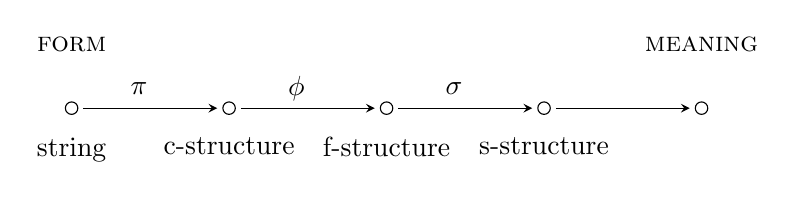
\begin{tikzpicture}
\draw[black] (0,0) circle (2.25pt) node[below=0.25cm] {string} node[above=0.6cm] {\sc form};
\draw[black] (2,0) circle (2.25pt) node[below=0.25cm] {c-structure};
\draw[black] (4,0) circle (2.25pt) node[below=0.25cm] {f-structure};
\draw[black] (6,0) circle (2.25pt) node[below=0.25cm] {s-structure};
\draw[black] (8,0) circle (2.25pt) node[above=0.6cm] {\sc meaning};
\draw [-stealth] (0.15,0) -- (1.85,0);
\draw [-stealth] (2.15,0) -- (3.85,0);
\draw [-stealth] (4.15,0) -- (5.85,0);
\draw [-stealth] (6.15,0) -- (7.85,0);
\node[text width=1cm] at (1.25,0.25) {$\pi$} ;
\node[text width=1cm] at (3.25,0.25) {$\phi$} ;
\node[text width=1cm] at (5.25,0.25) {$\sigma$} ;

\end{tikzpicture}
\caption{(Simplified) {\sc form-meaning} relationship in \citet[362]{kaplan1987three}}
\label{fig:ron_architecture}
\end{figure}

Proposals in the wider literature have assumed a slightly more complex representation of {\sc form}. Very early, \citet{Selkirk1984} proposed that syntactic structure is first mapped to a phonological (including prosodic) representation, which is then further processed by means of phonological rules and constraints before being mapped to a phonetic representation. In this model the string is not placed between the syntactic and the phonological module, but is the output of the phonological and the phonetic modules. Such a model is very much in line with psycholinguistic models of speech production and comprehension, e.g., as found in \citet{Levelt1999} and in \citegen{jackendoff2002foundations} work on Parallel Grammar; see \citetv{chapters/SimplerSyntax}. 

\begin{figure}
% \parbox{14cm}{
\footnotesize
\noindent ({\sc form})\hfill({\sc meaning})\\
\begin{tikzpicture}[baseline]
\matrix (a) [matrix of nodes, column sep=0.5cm, row sep=0.0cm, column 1/.style={anchor=base east}, column 2/.style={anchor=base west}, column 6/.style={column sep=0cm}, column 5/.style={column sep=0cm}]{
{\em comprehension} & Hearing & & Lexicon & & & \\
& & Phonology & & Semantics & {\hspace{2ex}\ } & Thought\\
{\em production} & Speaking & &  Syntax & & & \\
 };
\foreach \i/\j in {1-2/2-3}
    \draw[-stealth] (a-\i.east) -- (a-\j.west);
\foreach \i/\j in {2-3/3-2}
    \draw[-stealth] (a-\i.west) -- (a-\j.east);
\foreach \i/\j in {2-3/1-4,2-3/3-4,1-4/2-5,3-4/2-5}
    \draw[stealth-stealth] (a-\i.east) -- (a-\j.west);
\foreach \i/\j in {2-6/2-6}
    \draw[stealth-stealth] (a-\i.north east) -- (a-\j.north west);
\foreach \i/\j in {1-4/3-4}
    \draw[stealth-stealth] (a-\i.south) -- (a-\j.north);
\foreach \i/\j in {1-1/1-2,3-1/3-2}
   \draw[->,dashed] (a-\i.east) -- (a-\j.west);

\end{tikzpicture}
% }
\caption{The language processor \citep[cf.][197, modified]{jackendoff2002foundations}}
\label{fig:Jack}

\end{figure}

The model in \figref{fig:Jack} states clearly what is only implicitly expressed in theoretical LFG:\footnote{For example, in \figref{fig:ron_architecture} by means of arrows, and more explicitly in the pipeline architectures of the numerous computational LFG grammar implementations (see \citetv{chapters/ImplementationsApplications}).}
The different modules, placed between {\sc form} and {\sc meaning}, assume a certain directionality, generally termed as `comprehension' (parsing) and `production' (generation) in the wider literature. This is seemingly in conflict with the assumption that the different modules exist in `parallel' in LFG \citep[265]{DLM:LFG}; however, as Jackendoff explicitly remarks, this is not necessarily a hindrance:

\begin{quote}P[arallel] A[rchitecture] is nondirectional, but its constraints can be implemented in any order suited to particular processing tasks. \citep[589]{Jackendoff2010a}\end{quote}

\noindent `Parallel' under this approach refers to the general understanding that each module is subject to its own principles and constraints (= modularity). It does not mean that each component builds a completely isolated structure which then has to be aligned to the output of other modules. Instead, the individual constraints should be adjusted to the processing task at hand (which is either from {\sc form} to {\sc meaning} (comprehension/parsing) or from {\sc meaning} to {\sc form} (production/generation)). 

While this distinction might not carry much weight if a linguistic analysis is provided within one module of grammar (e.g., a syntactic phenomenon), it is crucial when modelling constraints at an interface, as the involvement of two (or more) modules always involves a `direction'. The assumptions made by Selkirk above, for example, are made from the perspective of production, while the architecture proposed by Kaplan in \figref{fig:ron_architecture} (and in general the vast majority of LFG-related linguistic analyses) is made from the comprehension perspective. The acknowledgement of this bidirectionality as made explicit in \figref{fig:Jack} is fundamental for the discussion of any interfaces between different modules, and thus essential for the proposals on the integration of prosody and its interfaces into LFG.
%is thus  crucial for the understanding of any proposal for integrating prosodic analysis into LFG.


Models which follow the parallel approach to prosody and its interfaces as detailed in \sectref{subsec:ps_interface} by assuming that modules are built up independently of each other and that their output is matched for the best alignment at each interface might seemingly be in line with the concept of modules existing in parallel. However, such models are not built to reflect the processing of a given speech signal to understand its meaning ($\rightarrow$\ comprehension), or the production of a signal expressing a specific thought ($\rightarrow$\ production).


%%%%%%%%%%%%%%%%%%%%%%%%%%%%%%%%%%%%%%%%%%%%%
%%%%%%%%%%%%%%%%%%%%%%%%%%%%%%%%%%%%%%%%%%%%%
%%%%%%%%%%%%%%%%%%%%%%%%%%%%%%%%%%%%%%%%%%%%%

%\include{files/previous_approaches}
\section{LFG approaches to prosody and its interfaces}
\label{sec:ps_LFG}

With respect to prosody and its interfaces, both the indirect reference and the parallel approach have been explored within the LFG community, mostly with a directional perspective. As these proposals frequently influence each other and furthermore represent very different views of grammar, the following section provides a chronological overview of the different approaches with a specific focus on the architectural assumptions behind each proposal. 

%%%%%%%%%%%%%%%%%%%%%%%%%%%%%
\subsection{From c-structure to p-structure: \citet{buttking98}}
\label{subsec:ButtKing}
\citet{buttking98} were the first to introduce a discussion of the syntax-prosody interface and p-structure to LFG. They assumed a mutually constraining model where d(iscourse)- and p-structure are projected off c-structure (in parallel to f-structure), as shown in \figref{Fig:archButtKing}.

\begin{figure}
\centering
{\small
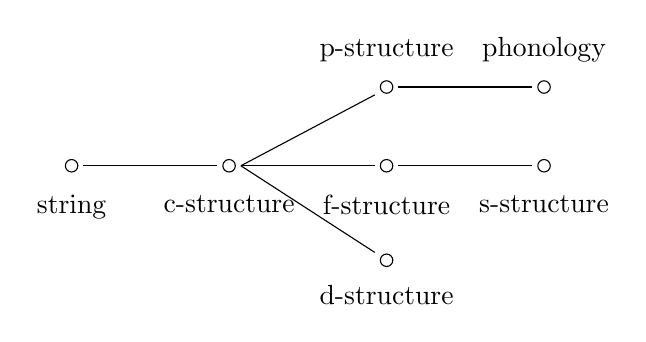
\begin{tikzpicture}


\draw[black] (4,1) circle (2.25pt) node[above=0.2cm] {p-structure};
\draw[black] (6,1) circle (2.25pt) node[above=0.2cm] {phonology};
\draw[black] (0,0) circle (2.25pt) node[below=0.25cm] {string};
\draw[black] (2,0) circle (2.25pt) node[below=0.25cm] {c-structure};
\draw[black] (4,0) circle (2.25pt) node[below=0.25cm] {f-structure};
\draw[black] (6,0) circle (2.25pt) node[below=0.25cm] {s-structure};
\draw[black] (4,-1.2) circle (2.25pt) node[below=0.2cm] {d-structure};
\draw  (0.15,0) -- (1.85,0);
\draw  (2.15,0) -- (3.85,0);
\draw  (2.15,0) -- (3.85,0.9);
\draw  (2.15,0) -- (3.85,-1.1);
\draw  (4.15,1) -- (5.85,1);
\draw  (4.15,0) -- (5.85,0);



\end{tikzpicture}
}
\caption{Grammar architecture according to \citet[][modified]{buttking98}}
\label{Fig:archButtKing}
\end{figure}

\noindent Under this approach, c-structure is a pivot point between d- and p-structure.\footnote{In contrast to this chapter which takes prosody to be part of phonology (see footnote 1), Butt and King differentiate between a p(rosodic)-structure and a phonological component.}
P(rosdic)-structure is viewed as an intermediate between c-structure and the phonological component itself which also contains postlexical phonological rules.

Based on work by \citet{HayesLahiri1991}, Butt and King focus on syntactically ambiguous sentences in Bengali, such as example (\ref{ex:ghost}).

\ea \label{ex:ghost}
\gll {ami} {bHut}  {dekH-l-am} \\
{I} {ghost} {see-{\sc pst}-{\sc 1sg}} \\
\glt a.\ \ `I was startled' \hspace{2ex}(idiomatic)\\
b.\ \ `I saw a ghost.' \hspace{1.5ex}(transitive)
\z

\noindent Following findings discussed in Hayes and Lahiri, Butt and King assume that prosody can be applied to differentiate between the idiomatic and the transitive interpretation.
For Bengali, the assumption for the syntactic-prosodic constituent mapping is that every clause is mapped to an Intonational Phrase ($\iota$,~IntP), every NP to a Phonological Phrase ($\varphi$,~PhP), and every main V or complex predicate is  phrased separately. \figref{fig:beng} shows the c-structures for (\ref{ex:ghost}) and the phrasing possibilities for {\em bHut dekHlam} which consist of separate phonological phrases in the transitive, and a single phonological phrase in the idiomatic reading.

\begin{figure}
\centering
\begin{minipage}{0.45\textwidth}

\hspace{2ex}Basic Transitive\\
\centering

%\vspace{1ex}
\begin{forest}
for tree={s sep=5mm, inner sep=0, l=0}
[S
    [NP
        [PRON\\ ami]
    ]
    [VP
        [NP
            [N\\ bHut\\ \hspace{2ex}(\hspace{4.5ex})$_{\varphi}$]
        ]
        [V$'$
            [V\\ dekHlam\\ \hspace{2ex}(\hspace{8.5ex})$_{\varphi}$]
        ]
    ]
]
\end{forest}
\end{minipage}
\begin{minipage}{0.45\textwidth}

\hspace{2ex}Idiomatic Reading\\
\centering

%\vspace{1ex}
\begin{forest}
for tree={s sep=5mm, inner sep=0, l=0}
[S
    [NP
        [PRON\\ ami]
    ]
    [VP
        [V$'$
            [N\\ bHut\\ \hspace{2ex}(\hspace{4.5ex})$_{\varphi}$]
            [V\\ dekHlam\\ \hspace{2ex}(\hspace{8.5ex})$_{\varphi}$]
        ]
    ]
]
\end{forest}
\end{minipage}
\caption{Two c-structure analyses for example (\ref{ex:ghost}), Butt and King (\citeyear{buttking98}, modified)}
\label{fig:beng}
\end{figure}

\citet{buttking98} represent p-structure as an AVM structure based on the prosodic hierarchy as shown in (\ref{ex:pros_hier_1}) above. The AVM structure allows for the inclusion of more detailed information beyond the prosodic domain and the p(honological)-form, such as pitch accents or boundary tones.  Butt and King also discuss the linearity issue given with any AVM approach. In order to apply phonological and phonetic processes, it is necessary to preserve the linear order of the string. For a possible solution to this issue, Butt and King point towards projection precedence \citep{zaenen-kaplan1995}, which arranges the attributes in p-structure similarly to the string.

\begin{sloppypar}
\figref{fig:idio_neut} shows the prosodic structure of the idiomatic reading in (\ref{ex:ghost}), where {\em bHut} and {\em dekHlam} are phrased into one phonological phrase ({\sc dom(ain): p-phrase}). 
\end{sloppypar}

\begin{figure}
{\small
\begin{center}
\avm[style=fstr]{
[dom & intonational-phrase\\
     & \{[dom & p-phrase\\
               & \{[ dom & p-word\\
                    p-form & \textup{ami} ]\}]\}\\
    & \{[dom & p-phrase\\
                & \{[ dom & p-word\hspace{0.5ex} \\
                    p-form & \textup{bHut}]\\
                   [ dom & p-word\\
                    p-form & \textup{dekHlam}]\}]\}\\



tone & high\\
bnd-tone & low\\]
}
\caption{Prosodic structure relating to the idiomatic reading in example (\ref{ex:ghost}), neutral focus}
\label{fig:idio_neut}
\end{center}
}
\end{figure}

The AVM includes all the information in the tree structure and the additional information known about the tones in the language, for example, that in a neutral (non-phonological) focus construction, a 
% neutral focus means that linear order and position determine the focus
high tone is associated with the left p-word in the rightmost p-phrase and the whole clause receives a low boundary tone. %As the information on tones is dependent on information from the grammar (information on focus), it is stored within the p-structure AVM. 
This information is stored in the AVM ({\sc tone high}), but the final association of the hight tone with the correct p-form (and the correct syllable in this p-form) is left to the phonological component itself. The reason is that the final p-phrase %(and with it the correct placement of the pitch accent in neutral focus) 
can only be identified once prosodic phrasing is complete and that the placement of the pitch accent  on the correct syllable is solely depending on the phonological structure of the word itself.

%(for Bengali, this is the first syllable of the prosodic word), 
Contrastive focus, on the other hand, is indicated by a low pitch accent and a high (intermediate) boundary tone at the level of the phonological phrase, as shown in \figref{fig:idio_contr}. As the target of the contrastive focus is determined by grammar (here d(iscourse)-structure), the associated pitch accent and boundary tone can be mapped to p-structure together with their domain. %Note that there is no distinction between the pitch accent and the boundary tone (or is this L*+H?).


\begin{figure}
{\small
\begin{center}
\avm[style=fstr]{
[dom & intonational-phrase\\
     & \{[dom & p-phrase\\
               & \{[ dom & p-word\\
                    p-form & \textup{ami} ]\}]\}\\
    & \{[dom & p-phrase\\
        tone & high\\
                & \{[ dom & p-word\hspace{0.5ex} \\
                    tone & low \\
                    p-form & \textup{bHut}]\\
                   [ dom & p-word\\
                    p-form & \textup{dekHlam}]\}]\}\\
bnd-tone & low\\]
}

\caption{Prosodic structure relating to the idiomatic reading in example (\ref{ex:ghost}), contrastive focus}
\label{fig:idio_contr}
\end{center}
}
\end{figure}

\newpage
Butt and King determine the tone distribution by using c-structure as a pivot between d-structure and p-structure, as shown in (\ref{ex:Prosody:6}).\footnote{For the interested reader: Focus in Bengali can also be signalled by the clitic -{\em o}. Following \citet{LahiriFitzpatrick-Cole1999}, Butt and King assume a lexical high tone which is introduced onto the prosodic word with the clitic's lexical specifications.}

\ea\label{ex:Prosody:6}
\begin{tabular}[t]{llll}
		  ($\downarrow_d$ {\sc focus-type}) &  =$_c$  & {\sc contrastive} & \\
		  ($\uparrow_p$ {\sc tone}) & = & {\sc high} & \hspace{4ex}$\rightarrow$\hspace{2ex} phrasal high\\
		  ($\downarrow_p$ {\sc tone}) & = & {\sc low} &  \hspace{4ex}$\rightarrow$\hspace{2ex} local low\\		  
\end{tabular}
\z



\noindent The approach proposed by \citet{buttking98} was later taken up in \citet{BoBuSu08} in their analysis of Urdu {\em ezafe}. In the {\em ezafe} construction in (\ref{ex:ezafebrackets}), the {\em ezafe} clitic is syntactically grouped with the following modifying noun, but is prosodically attached to the previous head noun.

\ea\label{ex:ezafebrackets}
\gll sher=e panjAb\\
lion=Ez  Punjab\\
\glt`a/the lion of Punjab'\\[1ex]
\begin{tabular}[t]{llll}
Syntactic Phrasing:  & [[sher] & {\bf [e} & panjAb]]\\
Prosodic Phrasing: & ((sher & {\bf e)} & panjAb)\\
\end{tabular}
\z

\noindent Example (\ref{ex:ezafebrackets}) shows a typical mismatch
between syntactic and prosodic structure, which is difficult to
account for if prosodic constituency is directly based on syntactic
constituency. The solution proposed in \citet{BoBuSu08} integrates the
{\em ezafe} clitic ({\sc cl-form}) into the phonological phrase using
a number of bookkeeping features to make sure an {\em ezafe} clitic is
present, as shown in \figref{fig:ezafe}.

\begin{figure}
\centering
{\small
\begin{minipage}{0.55\textwidth}
\begin{tabular}[t]{ll}
NPez$'$ $\longrightarrow$ \ N: & ($\uparrow_p$ {\sc dom}) = {\sc p-word}\\
 & ($\downarrow_p$ {\sc p-form}) = sher \\
 & ($\downarrow_p$ {\sc cl-form}) = ezafe \\
 &($\uparrow$ {\sc check} {\sc ezafe}) =$_c$ + \\[2ex]
 ezafe: & ($\uparrow$ {\sc check} {\sc ezafe}) = +
%&& \hspace*{.5em} ($\uparrow$ {\sc check conj}) ~= + \\
%&& \hspace*{.5em} $\downarrow_p$ \$ $\uparrow_p$ \\
\end{tabular}
\label{npezbar}
\end{minipage}
\begin{minipage}{0.4\textwidth}
%\epsfig{file=pics/ez_ps.eps,scale=.56}
{\footnotesize
\avm[style=fstr]{
[dom & p-phrase\\
     & \{[dom & p-word\\
               & \{[ p-form & \textup{sher} \\
                    cl-form & ezafe ]\}]\}\\
    & \{[dom & p-word\\
                & \{[ p-form & \textup{panjAb}]\}]\}\\
    ]
}
}

\end{minipage}
}
\caption{(Reduced) {\em ezafe} rule and the resulting p-structure in \citet{BoBuSu08}}
\label{fig:ezafe}
\end{figure}

This approach is not entirely satisfactory. For one, in this approach it is actually the noun which is `checking' for a following clitic, instead of the clitic `asking' to be grouped with a preceding prosodic host. Furthermore, this approach does not allow for a language-specific expression of prosodic principles, e.g., the general integration of {\em en}clitics into the preceding prosodic domain, and of {\em pro}clitics into the following prosodic domain. Instead, individual specifications have to be created for each clitic. This is not only unintuitive, but also does not allow for any predictions to be made about prosodic structure in general. 

Summing up, Butt and King make a first proposal to include prosodic information into LFG and show how this can interact with d- and c-structure. In contrast to \citegen{HayesLahiri1991} original approach (and in contrast to the claim made in \citealt{DLM:LFG}), their model does not permit the direct reference of phonological restructuring rules to relations internal to syntactic structure (e.g., to `right sister' or modifier-head-constructions), but provides an indirect, modular approach to the interface.

Butt and King distinguish between two structures: p-structure and the phonological component. P-structure only includes the information that is pre-deter\-mined by other modules of grammar, e.g., pitch patterns introduced by different sentence types and focus, and prosodic constituency based on syntactic constituency. This information serves as input to the phonological component (not further defined in their paper) and its inherent rules and constraints, which include prosodic restructuring, or the placement of pitch accents on the correct syllables within the right domains. %, but also possible rearrangements caused by clitic phenomena as found in \cite{Halpern95}.
This directional analysis from c-structure to p-structure to phonology reflects part of the production process in \figref{fig:Jack}. However, Butt and King's model (as shown in \figref{Fig:archButtKing}) is generally not in line with the architectural assumptions made in \figref{fig:ron_architecture} and \figref{fig:Jack} in that the string is not the representative of {\sc form}: neither is the string equal to the phonological output nor is it closely associated with the phonological module. Without this connection, it is unclear how the string could be realised in terms of a (physical) speech signal.

%%%%%%%%%%%%%%%%%%%%%%%%%%%%%%%%%%%%%%%%%%%%%
%%%%%%%%%%%%%%%%%%%%%%%%%%%%%%%%%%%%%%%%%%%%%
%%%%%%%%%%%%%%%%%%%%%%%%%%%%%%%%%%%%%%%%%%%%%

\subsection{Prosody and i-structure: \citet{Oconnor2005}}
\label{subsec:OConnor}
In his thesis, \citet{Oconnor2005} discusses the interface between prosody and information structure.
\citet{Oconnor2005} assumes a bidirectional approach, which distinguishes between a `hearer-based'  and a `speaker-based' approach. He explicitly focusses only on the hearer-based direction (from p- to d-structure $\rightarrow$ comprehension) and leaves the speaker-based direction (from d- to p-structure $\rightarrow$ production) to further research.

\largerpage
O'Connor's approach is based on the AM/ToBI framework (see \sectref{subsec:what_pros}), but the description of accents is restricted to High and Low tones only.\footnote{O'Connor does not distinguish  between different types of pitch accents and how these may relate to specific i-structure categories, e.g., the distinction between broad and narrow focus based on different pitch patterns \citep[a.o.,][]{Baumannetal2007}.} %p.35
%Goldsmith1976,
He is mostly concerned with utterances where a difference in meaning is expressed solely by means of prosodic emphasis (expressed by capital letters in example (\ref{ex:dragon})).

\ea\label{ex:dragon}
\ea\label{ex:dragona} He rode [a green DRAGON]\textsubscript{\textit{foc}}.
\ex\label{ex:dragonb} He rode a [GREEN]\textsubscript{\textit{foc}} dragon.
\z\z


\noindent The two propositions have a different information structure. Example (\ref{ex:dragona}) can be the answer for a question with a broad focus (e.g., {\em Did he ride a green dragon or a thestral?}\/), while example (\ref{ex:dragonb}) is more likely to be the (contrastive) answer to a question like {\em Did he ride a green dragon or a blue dragon?}

In his proposal, O'Connor assigns a central role to i-structure. 
As the AM/ToBI system is not concerned with the influence of syntactic structure on prosody, 
 O'Connor assumes that prosody and i-structure can be related to each other without syntactic mediation, as shown in \figref{fig:Prosody:OConnor}.\footnote{O'Connor does not completely exclude the influence of c-structure on prosody, but only acknowledges a relevance of the linear and hierarchical syntactic structure of the clause for  the length of the transition between tonal events and the alignment of the pitch in general.}

\begin{figure}
\centering
\begin{tikzpicture}[baseline]
\matrix (a) [matrix of nodes, column sep=0.75cm, row sep=0.0cm, column 1/.style={anchor=base east}, column 3/.style={anchor=base west}]{ 
& & p-structure\\
d-structure & i-structure & c-structure \\
& & lexicon/morphology\\
 };
\foreach \i/\j in {2-2/2-3,2-2/1-3,2-2/3-3}
    \draw[-stealth] (a-\i.east) -- (a-\j.west);
\foreach \i/\j in {2-1/2-2}
    \draw[stealth-stealth] (a-\i.east) -- (a-\j.west);

\end{tikzpicture}
\caption{Architecture proposed in \citet[Fig 6.3, 142, modified]{Oconnor2005}}
\label{fig:Prosody:OConnor}
\end{figure}

\noindent Following the general idea behind autosegmental approaches \citep{Goldsmith1976}, O'Connor pursues the idea of a representation of tonal information independent from the segmental/phonemic representation. 
He proposes that p-structure should be represented by a hierarchical constituent structure (thus paralleling c-structure). Via so-called `tune structure rules' like the ones in (\ref{ex:Prosody:9}), a tree-like structure is created to represent intonation where the terminal nodes correspond to underspecified tonal events: t$^{*}$ represents a pitch accent, t$^-$ a phrase accent, and t\% a boundary tone.

\ea\label{ex:Prosody:9}\begin{itemize}
    \item[] n $\geq$ 1
    \item[a.] {\sc Tune}$_{IP}$\ $\rightarrow$\ \ tune$_{ip}^n$\ \  t\%
    \item[b.] \hspace{0.4ex}tune$_{ip}$   \hspace{1.2ex} $\rightarrow$\ \ t$^{*n}$\hspace{3ex} \  t$^-$
    \end{itemize}
\z

\noindent As a result, each prosodic tree constructed on the basis of these rules has four obligatory nodes: the prosodic `intermediate phrase' ({tune}$_{ip}$) consists of a nuclear accent t* and a phrase accent t$^-$ while the prosodic `intonational phrase' ({\sc tune}$_{IP}$) consists of at least one intermediate phrase and a boundary accent t\%.
For example (\ref{ex:ghost}) (see also \figref{fig:beng}, basic
transitive) from \citet{buttking98}, O'Connor proposes the p-structure in \figref{fig:connor}.

\begin{figure}
  \centering
  \includegraphics[width=.55\textwidth]{figures/Prosody/Boegel_Figure_12.pdf}
\caption{O'Connor's p-structure as applied to example (\ref{ex:ghost}) from \citet{buttking98}}
\label{fig:connor}
\end{figure}

The tree representation is mainly concerned with the organisation of tonal events; the material below the dashed line includes the orthographic tier and the prosodic domain information in the form of bracketing.\footnote{As \citegen{Oconnor2005} main focus is on the relation between intonation and discourse functions, the encoding of further prosodic/phonological information, e.g., syllable structure, or lexical stress, is not further discussed in his thesis.}


O'Connor emphasises the point that under his approach, the association of the High tone is not left to a further phonological component as proposed in \citet{buttking98} and discussed above in \sectref{subsec:ButtKing}. It is however not quite clear how the High tone is associated with the correct string sequence in O'Connor's approach, as no formal  alignment of string and pitch (i.e., c-structure and p-structure) is established in his thesis. Indeed, in the data provided by Butt and King, the High tone should be assigned to the `leftmost' prosodic word in the `rightmost' phonological phrase. As O'Connor collapses all three phonological phrases proposed by Butt and King under one tune$_{ip}$, it is not clear how the association of the High tone with the correct word can be ensured.

With respect to i-structure, O'Connor assumes that categories like {\sc focus} and {\sc topic} are organised linearly in an utterance, and assigns each to one tune$_{ip}$, as shown in (\ref{ex:Prosody:10}). If there are not enough tunes, then the assumption is that there is no topic correspondent.

\ea\label{ex:Prosody:10}
\phraserule{{\sc Tune}$_{IP}$}{
  \rulenode{tune$_{ip}$\\{$\downarrow\ \in \{\uparrow_d$\ {\sc topic}\}}}
  \rulenode{tune$_{ip}$\\{$\downarrow\ \in \{ \uparrow_d$\ {\sc focus}\}}}
  \rulenode{t\%}}
\z

\noindent As O'Connor notes, there are a number of cases where the proposed association of i-structure categories and tunes does not work. Sentences like {\em `It broke.'} will only have one tune, indicating a {\sc focus}. However, in i-structural terms, {\em It} is a {\sc topic}. This mismatch between tunes and i-structure roles is discussed \citep[161]{Oconnor2005}, but not resolved.

In conclusion, O'Connor's indirect, directional approach to the relationship between prosody and i-structure suggests an alternative to the syntactocentric view proposed in \citet{buttking98}.  However, there are a number of outstanding questions. Besides the incomplete association of i-structure categories to tune-structure rules  just discussed, there is also the fundamentally important question as to how tonal events can be associated with their targets without reference to the morphosyntactic string, or how common phenomena, e.g., the (syntactic) scope of a prosodically expressed focus, can be determined without reference to syntactic constituency. The missing association of p-structure, string, and c-structure, and other unresolved questions thus only allow for an analysis of a more descriptive nature.

%%%%%%%%%%%%%%%%%%%%%%%%%%%%%%%%%%%%%%%%%%%%%
%%%%%%%%%%%%%%%%%%%%%%%%%%%%%%%%%%%%%%%%%%%%%
%%%%%%%%%%%%%%%%%%%%%%%%%%%%%%%%%%%%%%%%%%%%%
\subsection{The string as an interface between c- and p-structure: \citet{boegeletal09,boegel-etal2010}}
\label{subsec:Boegeletal}
%Following discussions in \cite{WheeldonLahiri1997} (see also \cite{Mycock2006},, 
Based on the realisation  that the frequent misalignment of prosodic and syntactic constituents would seriously complicate previously established prosody-syntax mapping algorithms, \citet{boegeletal09} pick up on the notion of the parallel approach discussed in \sectref{subsec:ps_interface}. The underlying assumption is that the prosodic component operates independently of syntax and that the two components are not related via LFG's projection architecture. To account for the cases where syntax is influenced by prosody, \citet{boegeletal09} assume  a directional `pipeline' architecture (from the comprehension perspective): First, an independent prosodic component interprets various phonological properties thus establishing the boundaries of prosodic units.  This information on prosodic constituency is then made available to syntax by inserting prosodic  bracketing features into the terminal string of c-structure.\footnote{Under this approach, the string has a central role as it includes information from both the syntactic and the prosodic component (similar to the understanding of the string in \citealt[110]{Asudeh2009} as a `linear representation of phonology').}  

\citet{boegeletal09} discuss a number of different phenomena, among them Urdu {\em ezafe} \citep[see \sectref{subsec:ButtKing}]{BoBuSu08}. They extend the c-structure rules by adding left and right prosodic brackets (`lexical categories' RB and LB) which reflect prosodic constituency.

\ea\label{rule:extended}
\ea \phraserule{\makebox[2.4em][l]{EzP}}{EZ ~ RB ~ N}
\ex \phraserule{NPez$'$}{LB ~ [$\ldots$] ~N}
\z
\z

\noindent The inclusion of brackets greatly simplifies the rule originally used in \citet[Figure 10]{BoBuSu08} where a number of {\sc check}-features were applied to control for an {\em ezafe} clitic following the head noun. The resulting c-structure representation, shown in \figref{fig:Prosody:11}, allows for the depiction of the misalignment between syntactic and prosodic structure.


\begin{figure}
\centering
%\vspace{1ex}
{\footnotesize
\begin{forest}
for tree={s sep=5mm, inner sep=5, l=0}
[NP
    [LB\\ (,tier=term]
    [NPez, l=10
        [NPez$'$
            [LB\\ (]
            [N\\ sher,tier=term]
        ]
        [EzP
            [EZ\\ e]
            [RB\\ )]
            [N\\ panjAb]
        ]
    ]
    [RB\\),tier=term]
]
\end{forest}
}
\caption{Urdu {\em ezafe} analysis as proposed in \citet{boegeletal09}}
\label{fig:Prosody:11}
\end{figure}

\noindent Another aspect discussed in \citet{boegeletal09} is the prosodic resolution of syntactically ambiguous structures. Consider the following example, where {\em old} can either modify only the first noun ((\ref{ex:oldmen}a)) or scope over the whole coordination ((\ref{ex:oldmen}b)). Each possibility is accompanied by a distinct prosodic grouping.

\ea\label{ex:oldmen}\begin{itemize}
\item[a.] \gll {[old men]} and [women]\\
{(old men)} and (women)\\
\glt {\ }

\item[b.] \gll [old [men and women]]\\
(old (men and women))\\
\glt
\end{itemize}
\z

\noindent The paper postulates a `Principle of Prosodic Preference', according to which the syntactic component  disprefers syntactic structures whose constituent boundaries do not coincide with prosodic boundaries. For the implementation, \citet{boegeletal09} use a metarule, which systematically transforms the rules of the syntactic component. In the following metarule, CAT is a nonterminal category, and RHS denotes the regular language over categories which are annotated with co-describing constraints.

\ea
   \phraserule{CAT}{RHS}
\z

\noindent In Bögel et al.'s metarule in (\ref{ex:meta}), the top part of the rule will match a (recursive) sequence of CAT surrounded by prosodic brackets (LB and RB). The bottom part will match the RHS regular expression if all occurrences of LB or RB are ignored, thus preventing the inserted prosodic brackets from ruling out a valid syntactic analysis.\footnote{The `Ignore operator' / was first introduced in \citet{KaplanKay1994}.}


\ea\label{ex:meta}\ 

\vspace{-4.1ex}
\begin{tikzpicture}[baseline]
\matrix (a) [matrix of nodes, column sep=0.5cm, row sep=0.0cm]{
CAT & $\rightarrow$ & LB\ \  CAT\ \  RB\\
& & \textbar \ RHS / [ LB \textbar\ RB ]\\
& & \hspace{10ex}Disprefer\\
 };
\end{tikzpicture}
\z

\noindent The Principle of Prosodic Preference is enforced via the `Disprefer' optimality mark,\footnote{See \citetv[section~\ref{sec:runtime_performance}]{chapters/ImplementationsApplications} for a description of optimality marks and relevant references.} %
which assigns a dispreference mark to the construction every time the bottom part of the metarule in (\ref{ex:meta}) is applied. In the case of several possible syntactic analyses (as in (\ref{ex:oldmen})), this extension effectively ranks the analyses: The top half of the rule only applies if the prosodic brackets match the syntactic structure, while the syntactic analyses with no matching prosodic brackets will be parsed by the bottom half of the rule, but will receive a `Disprefer' mark. This allows for constructions with matching prosodic and syntactic brackets to be preferred, while constructions with non-matching brackets will only be valid if a preferred solution (with matching brackets) is not available.


This first approach to the interface was extended in \citet{boegel-etal2010} which discusses second position (2P) clitics in Russian and Serbian/Croation/Bosnian (SCB). It is concerned with examples like (\ref{ex:SCB1}), where a clitic cluster (CCL) disrupts the NP {\em Taj \v{c}ovek}. 


\ea\label{ex:SCB1}
\gll 
{[}Taj {\em joj} {\em  ga} {\em je} \v{c}ovek]  poklonio. \\
\phantom{[}that her it {\sc aux} man presented\\
\glt `That man presented her with it.' \hfill \citep{Schuetze1994}
\z

\noindent These clitics appear in the second position after a first prosodic word without regard to syntactic requirements ((\ref{ex:SCB1_pros})).

\ea\label{ex:SCB1_pros}
\gll
(((Taj)$_{\omega}$ ({\em joj}  {\em ga}  {\em je})$_{cl}$)$_{\omega}$ (\v{c}ovek)$_{\omega}$)$_\varphi$ (poklonio)$_\varphi$\\
\phantom{(((}That \phantom{(}her it {\sc aux} \phantom{(}man \phantom{(}presented\\
\glt`That man presented her with it.'
\z

\noindent Such a structure is problematic for traditional LFG accounts, because it is difficult to account for the clitics' appearance within an NP and to furthermore retrieve the clitics' functional contribution to the clausal f-structure. With a purely syntactic account, this information is locked into the NP's f-structure.

\citet{boegel-etal2010} resolve this issue by assuming a shared responsibility between the syntactic and the prosodic component: While the syntactic component ensures the availability of the functional information by placing the clitic in the (linear) first position, the prosodic component ensures the correct position of the clitics within the clause and places the clitics following the first prosodic word. This prosodic repair mechanism has been shown to apply crosslinguistically and was dubbed `prosodic inversion' by \citet{Halpern95}.\footnote{For further work in LFG, see an account of prosodically determined second position clitics in Vafsi in \citet{Boegeletal2018}.}

In order for the clitic to appear in the correct syntactic position, \citet{boegel-etal2010} define the rule in (\ref{modifiedS}), where  RHS$_S$ denotes the possible expansion of the clausal S node with left and right brackets (as discussed above).   LB$_S$ is a pre-terminal node that marks the left edge of a clause and allows syntactic/prosodic constraints to be aligned with respect to clause boundaries. CCL can optionally appear as a prefix to the S expansion; the $\uparrow$=$\downarrow$ annotation ensures the processing of the clitics' clause-level functional information.


\ea\label{modifiedS}
\phraserule{S}{LB$_S$
  \rulenode{(CCL)\\\UP=\DOWN}
  RHS$_S$}
\z

\noindent To account for the prosodic placement, \citet{boegel-etal2010} distinguish between a prosodic and a syntactic (c-structure terminal) string which includes the lexical formatives discussed above. The interface between these (usually aligned) strings is a regular relation, where the syntactic string is the `upper language' and the prosodic string is represented by the `lower language'. In the simplified illustration in (\ref{regrel}), the upper language/syntactic string clitic sequence (CS:0) immediately following the clause boundary ($_S$ is placed after the first prosodic word $\omega$ in the prosodic string  in the lower language/prosodic string (0:CS). 

\ea\label{regrel} 
\begin{tabular}[t]{lllcl}
s(yntactic)-string (`upper'): & ($_S$ & CS & $\omega$ & 0 \\[0.5ex]
\hline
& & & & \\[-2.2ex]
p(rosodic)-string (`lower'): & ($_S$ & 0 & $\omega$ & CS  \\
\end{tabular}
\z


\noindent The regular relation has the effect that strings with syntactically clause-initial clitic sequences are related to strings where those clusters appear on the other side of an adjacent prosodic word. The sentence-initial position allows for the functional information to be made available to syntax, but violates the prosodically dependent clitic's need for a preceding host.
The second position in the prosodic string satisfies this prosodic constraint in that the clitic is placed following a valid prosodic host.

\begin{figure}
  \centering
  \includegraphics[width=.6\textwidth]{figures/Prosody/Boegel_Figure_14-cstr.pdf}
  \raisebox{2cm}{\scalebox{.8}{\avm[style=fstr]{
  [pred & `present\arglist{subj,obj,obj2}'\\
    subj & [pred & `man'\\
      pers & 3\textsubscript{\textnormal{\footnotesize\textit{je}}}\\
      num & sg\textsubscript{\textnormal{\footnotesize\textit{je}}}\\
      spec & that]\\
    obj$_{ga}$ & [pred & `pro'\\
      pers & 3\\
      num & sg\\
      gend & masc]$ga$\\
    obj2\textsubscript{\textnormal{\footnotesize\textit{joj}}} & [pred & `pro'\\
      pers & 3\\
      num & sg\\
      gend & fem]{\textnormal{\textit{joj}}}\\
     tense & past\textsubscript{\textnormal{\footnotesize\textit{je}}}]
    }}}
\caption{2P clitics and the syntax-prosody interface \citep[13]{boegel-etal2010}}
\end{figure}


\noindent In conclusion, \citet{boegeletal09} set up a directional architecture where they assume an independent prosodic component to process information related to prosody. Information on prosodic constituency is only entered into the terminal syntactic string in the  form of lexical formatives, that is, the approach pursues a softer version of the parallel approach discussed above in \sectref{subsec:ps_interface}. This allows for an account of general prosody-syntax misalignment, but also for a prosodic resolution of syntactically ambiguous structures. The approach was furthermore extended to account for second position clitics as well.

There are also several problems with this approach. For one, no further prosodic information can be transmitted via the string. However, information on pitch patterns, accent types or other prosodic features can be crucial for a correct interpretation of meaning. 

\begin{sloppypar}
Another factor is the relatively coarse-grained representation of prosody. Prosodic units can be relevant down to the syllable, a granularity that becomes difficult to represent by interspersing brackets with the terminal c-structure string.
And finally, integrating the prosodic structures into the c-structure analysis makes the representation not only difficult to process, but is also questionable in terms of modularity.
\end{sloppypar}

%%%%%%%%%%%%%%%%%%%%%%%%%%%%%%%%%%%%%%%%%%%%%
%%%%%%%%%%%%%%%%%%%%%%%%%%%%%%%%%%%%%%%%%%%%%
%%%%%%%%%%%%%%%%%%%%%%%%%%%%%%%%%%%%%%%%%%%%%
\subsection{A stricly parallel approach: \citet{DM11}, \citet{MycockLowe2013}}
\label{subsec:Dalrympleetal}

Dalrymple, Mycock, and Lowe base their approaches\footnote{The approach to the interface described in this section was developed in a number of works, namely \citet{Mycock2006, DM11, MycockLowe2013} (see also \citealt{lowe:16a} and \citealt{Jones2016} for further discussion); the version described here is part of the prosody chapter in \citealt{DLM:LFG}.} on the assumption that the prosodic and the syntactic component are parallel but separate components, which goes beyond the distinction between direct and indirect approaches to prosody and its interfaces as briefly discussed in \sectref{subsec:ps_interface}. In the parallel approach, syntactic structure has no influence on the formation of prosodic structure (and vice versa).\footnote{\citet[398]{DLM:LFG} classify their approach as indirect reference. However, all indirect reference approaches include syntactic structure as a main factor for building up prosodic structure (mostly from the perspective of production). This is not the case here.} Instead, each structure is built up independently: syntactic structure as traditionally assumed, and prosodic structure based on rhythmic principles, more specifically, the trochaic foot. In constrast, the indirect reference approach assumes that rhythmic structure is only one factor among many which contribute to the formation of prosodic structure.

The approach represents prosodic constituency in a tree-like structure, assuming the constituents proposed by \citet{Selkirk1995} (see \sectref{subsec:what_pros}). Similar to the proposal made in  \citet{boegel-etal2010}, the interface between the syntactic and prosodic components is the interface between a s(yntactic)-string and a p(honolog\-i\-cal)-string. The ``linguistic signal'' (\citet[][407]{DLM:LFG}, the nature of which is not further defined) is parsed into minimal syntactic units in the s-string, and into minimal prosodic units (i.e., syllables) in the p-string.
A (very simplified) representation of the example sentence {\em Anna was studying at the university} is shown in \figref{fig:simple} (see \figref{fig:compl} for a complete picture).

\begin{figure}
\centering
(c-structure)\\
... \\
\begin{tikzpicture}[baseline]
\matrix (a) [matrix of nodes, column sep=0cm, row sep=0.2cm]{
%& \multicolumn{6}{c}{\small (c-structure)}\\
& {N} & {I} & {V} & {P} & {D} & {N} \\
& \hspace{-3ex}$\pi$ & \hspace{-3ex}$\pi$ &\hspace{-3ex}$\pi$ &\hspace{-3ex}$\pi$ &\hspace{-3ex}$\pi$ &\hspace{-3ex}$\pi$ \\
\hspace{-23.7ex}s-string: & {\em Anna} & {\em was} & {\em studying} & {\em at} & {\em the} & {\em university}\\
};

\foreach \i/\j in {3-2/1-2,3-3/1-3,3-4/1-4,3-5/1-5,3-6/1-6,3-7/1-7}
    \draw[-stealth] (a-\i.north) -- (a-\j.south);
    
\begin{scope}[yshift=-4cm]
\matrix (b) [matrix of nodes, column sep=0cm, row sep=0.2cm, row 4/.style={row sep=0.4cm}, row 3/.style={row sep=0.5cm}, row 5/.style={row sep=0.6cm}, column 1/.style={column sep=0.5cm}]{
%& \multicolumn{6}{c}{\small (c-structure)}\\
\hspace{-5.25ex}p-string: & {\ae} & {n\textschwa} & {w\textschwa z}& {stʌ} & {di} & {\textsci{\ng}} & {\textschwa t} & {{\dh}\textschwa} & {ju} & {n\textschwa} &{vɜ:} &{s\textschwa} & {ti}\\

& \hspace{-3ex}$\beta$ & \hspace{-3ex}$\beta$& \hspace{-3ex}$\beta$& \hspace{-3ex}$\beta$& \hspace{-3ex}$\beta$& \hspace{-3ex}$\beta$& \hspace{-3ex}$\beta$& \hspace{-3ex}$\beta$& \hspace{-3ex}$\beta$& \hspace{-3ex}$\beta$& \hspace{-3ex}$\beta$& \hspace{-3ex}$\beta$& \hspace{-3ex}$\beta$\\

 & {S} & {S} & {S} & {S} & {S} & {S} & {S} & {S} & {S} & {S} & {S} & {S} & {S}\\
 
 & & {PW} & & & & & {PW} & & & & & {PW} &\\
 
 & & {PhP} & & & & & {PhP} & & & & & {PhP} &\\
 
& & & & & & & {IntP} & & & & & &\\
};
\end{scope}
\foreach \i/\j in {3-2/1-2,3-2/1-3,3-3/1-4,3-4/1-5,3-4/1-6,3-4/1-7,3-5/1-8,3-6/1-9,3-7/1-10,3-7/1-11,3-7/1-12,3-7/1-13,3-7/1-14}
  \draw[dashed] (a-\i.south) -- (b-\j.north);
\foreach \i/\j in {1-2/3-2,1-3/3-3,1-4/3-4,1-5/3-5,1-6/3-6,1-7/3-7,1-8/3-8,1-9/3-9,1-10/3-10,1-11/3-11,1-12/3-12,1-13/3-13,1-14/3-14}
 \draw[-stealth] (b-\i.south) -- (b-\j.north);
\foreach \i/\j in {4-3/3-2,4-3/3-3,4-3/3-4,4-8/3-5,4-8/3-6,4-8/3-7,4-8/3-8,4-8/3-9,4-8/3-10,4-8/3-11,4-13/3-12,4-13/3-13,4-13/3-14}
 \draw (b-\i.north) -- (b-\j.south);
\foreach \i/\j in {4-3/5-3,4-8/5-8,4-13/5-13,5-8/6-8,5-3/6-8,5-13/6-8}
\draw (b-\i.south) -- (b-\j.north);


\end{tikzpicture}
\caption{Simplified interface for {\em Anna was studying at the university} \citep[][408, showing only c-structure terminal nodes]{DLM:LFG}}%example tree (DM 2011, amended to fit ML2013, p.408, example 17)}
\label{fig:simple}

\end{figure}

\figref{fig:simple} displays the syntactic component (s-string and c-structure) in the top part. The bottom part represents p-structure: the p-string and the prosodic tree. The p-string is parsed into syllables (but see below for further specifications) which are grouped into prosodic words. Following \citet{LahiriPlank2010}, prosodic structure is built based on rhythmic principles, specifically on the trochaic foot (see \sectref{subsec:ps_interface}). The representation omits the foot structure, but the 
underlying formation algorithm is still visible in the fact that the left edge of each prosodic word is placed with the syllable carrying primary stress in a lexical, (syntactic) word; e.g., u.ni.(VER.si.ty)$_{\omega}$. Function words and feet built on secondary stress (e.g., (ˌu.ni)$_{ft}$) seem to generally be phrased with the preceding prosodic word.\footnote{It would be interesting to see how this approach can be applied to cases where the first syllable of a prosodic unit is unstressed as in a modified version of example (\ref{ex:AnnaUni}), {\em Anna or Ravi and Karla  ...} (Anna $\vee$ (Ravi $\wedge$ Karla)), where the prosodic boundary is realised directly after {\em Anna} \citep{Wagner2010}, while the rhythmic approach would predict the prosodic boundary to occur after {\em or}.} The following example shows the prosodic phrasing according to a trochaic foot structure, with primarily stressed syllables in capital letters.

\ea\label{ex:AnnaUni}{(Anna was) (STUdying at the uni) (VERsity)}
\z


\noindent The formation of prosodic words based on rhythmic principles naturally leads to regular mismatches between syntactic and prosodic units. 
However, the approach raises the question whether these units are indeed prosodic words or whether they should rather be defined as phonological phrases. If these units are prosodic words, then the question arises how phonological phrases are defined under this approach. In \figref{fig:simple}, each phonological phrase is identical with a prosodic word, which is a crosslinguistically very unusual 1-1 relationship.\footnote{See, for example, the family of {\sc BinMin}-constraints, which require for a higher prosodic domain to contain more than one unit of a lower prosodic domain \citep[a.o.,][]{Ghini1993, InkelasZec1995}.}


\citet{MycockLowe2013} extend the string interface by assuming that the string-units are not atomic but should rather be seen as feature bundles, represented as AVMs.
The relation between the two strings and their units is regulated through information stored in the lexicon. While the lexical s(yntactic)-form contains the traditional morphosyntactic information, the p(honological)-form contains information on segments and syllable structure as well as the feature {\sc syllstress} which indicates the primary lexical stress position. 

In addition to the lexical information, the feature structures at the interface also include information on the edges of constituents in the respective modules. These `edge features' are necessary to allow for the matching of prosodic and syntactic constituents, e.g., in order to prosodically disambiguate syntactically ambiguous structures. Mycock and Lowe define a number of mechanisms to make the edges available to the strings: $\Swarrow$ and $\Searrow$ for the left and right edges of syntactic nodes, and $\Prosleftarrow$ and $\Prosrightarrow$ for the left and right edges of prosodic nodes.\footnote{See \citet{DLM:LFG} for the exact definitions.} \figref{fig:avmsAnna} shows the AVMs for the first syntactic and the first prosodic unit of example (\ref{ex:AnnaUni}), where the values of {\sc l}(eft) and {\sc r}(ight) consist of a set of syntactic and prosodic nodes whose edges are represented by this particular form.  

\begin{figure}
\begin{tabular}{cc}
  s-string unit {\em Anna} & p-string unit {\em\ae}\\
\avm[style=fstr]{
[ fm & Anna \\
 L & \{ IP, NP, N \} \\
 R & \{ NP, N \} \\
]
}
&
\avm[style=fstr]{
[  fm & \textup{\ae} \\
syllstress & P \\
 L & \{ IntP, PhP, PW \} \\
 R & \{ \ \} \\
]
}
\end{tabular}
\caption{Feature structure for first unit of the p-string and the s-string \citep[][412]{DLM:LFG}}
\label{fig:avmsAnna}
\end{figure}

\noindent
At the interface, a ``Principle of Interface Harmony'' ensures that the best-match\-ing parses between the p-string and the s-string are preferred. Note, however, that the approach does not explain how this preference is implemented.\footnote{\citet{lowe:16a} presents a possible implementation of the Principle of Interface Harmony using additional formal power in form of OT contraints (see also \citealt{LoweBelyaev2015}). A critical discussion of this approach can be found in \citet[][Ch.6]{Boegel2015}.}

Furthermore, the question of which syntactic and prosodic constituent edges should be matched, that is, which prosodic boundary type is important to syntax and vice versa, is left for future research \citep[][419]{DLM:LFG}. This is surprising, given the extensive existing literature on the topic, but in a sense it is a necessary consequence of assuming strictly parallel modules as has been discussed in \sectref{subsec:ps_interface}.

Apart from the interface to syntax, the string interface also serves as an interface between prosody and semantics and i-structure.\footnote{As the description of the interface to i-structure is similar to the one provided for the prosody-semantics interface, the interested reader is referred to \citet{DLM:LFG} for details.} The semantics-prosody interface is demonstrated by means of declaratives, where the intonational contour distinguishes between declarative statements and questions. In order to make the semantic information available at the string interface, the c-structure receives a ``label'' PolarIntSem along with the meaning constructor [PolarInt]. Similar to the edge values, this label is handed down to the s-string where it is placed in the rightmost AVM.

For the prosodic interpretation of a declarative question, information on pitch is required. This information is included in the form of H and L pitch accents and boundary tones. 

\citet{DLM:LFG} assume that in English declarative questions, a nuclear L tone is associated with the stressed syllable of the first prosodic word in the last phonological phrase, and an H boundary tone at the right edge of the Intonational Phrase.\footnote{The prosodic expression of declarative questions in English shows much more variability than assumed here, see, e.g., \citet{Gunlogson2003} for discussion of different contours.} Similar to \citet{Oconnor2005} above (\sectref{subsec:OConnor}), they annotate prosodic structure by means of prosodic phrase structure rules. In addition, a label {\em PolarInt} appears at the rightmost AVM of the p-string.
The rule in (\ref{ex:MLrule}) can then be read as follows: In this phonological phrase, assign a nuclear tone L to the leftmost syllable with primary stress ($\Prosleftarrow^{s}$) and a right boundary tone to the rightmost unit;\footnote{The assignment of a right boundary tone here does not distinguish between `boundary tones', e.g. H\%, which appear as boundary tones of intonational phrases, and `phrase accents', e.g., H$^-$, which appear at the edges of phonological phrases. If both edges fall together, these tones form combinations, e.g. H-H\%, which can be crucial for an interpretation. The use of a boundary tone with a phonological phrase unfortunately collapses this distinction.} if these constraints are satisfied, create a label {\em PolarInt} which appears as a set member of the rightmost unit's right edge.

\ea\label{ex:MLrule}
\phraserule{IntP}{
  PhP*
  \rulenode{PhP\\
(($\Prosleftarrow^{s}$ {\sc n\_tone}) = L)\\
($\Prosrightarrow$ {\sc rb\_tone}) = H $\Rightarrow$\\
{\em PolarInt} $\in$ ($\Prosrightarrow${\sc r})}}
\z

\noindent \figref{fig:compl} shows part of the full analysis for example (\ref{ex:AnnaUni}), the PP {\em at the university}. In addition to the edge features, both labels, PolarIntSem and {\em PolarInt}  appear at the right edge of the string interface. The Principle of Interface Harmony requires both labels to co-occur for the overall structure to be grammatical, but the matching process is not further detailed here.

\begin{figure}[p]
\includegraphics[width=\textwidth]{figures/Prosody/Boegel_Figure_17.pdf}
\caption{Analysis of the PP in the declarative question {\em Anna was studying at the university?}\label{fig:compl}}
\end{figure}

In conclusion, the non-directional model proposed by \citet{DLM:LFG} pursues the idea of modularity in the extreme: the syntactic and the prosodic component are taken to be completely independent  structures which do not allow for any co-description mechanisms as commonly found in LFG (see \citetv{chapters/CoreConcepts}).
Instead, information about (at least) syntactic and prosodic constituency, semantics, i-structure, and intonational contours is handed to the respective strings. The interface between the syntactic and the prosodic component is then situated between the s-string and the p-string, where matching edges and `labels' are preferred according to the Principle of Interface Harmony. 

Apart from initial suggestions involving OT-constraints in \citet{lowe:16a} and \citet{LoweBelyaev2015}, the formal implementation of the Principle of Interface Harmony is not further detailed. Given that there are numerous combinatorial possibilities of prosodic constituents, pitch accents, phrase accents, and boundary tones, and hardly any of them can be mapped to one particular interpretation, but are always co-dependent on other modules of the grammar, the matching of labels at the string interface will most likely prove to be difficult.
The introduction of these labels and the mingling of information from different modules is, however, a necessary consequence of the parallel approach. The reduction of the interface to the strings implies that {\em all} potentially relevant information from other modules has to be duplicated and appear as part of the string where it might or might not be matched against the material in the parallel string. As it was the case in \citet{boegeletal09,boegel-etal2010} (\sectref{subsec:Boegeletal}), this is also problematic with respect to modularity.

The extensive duplication and blending of structures can be avoided by assuming a more traditional co-descriptive approach, while at the same time acknowledging modularity in that each module only processes information related (i.e., `native') to its module. This indirect reference approach was first pursued in \citet{buttking98}, and was further developed in \citet{Boegel2015} and subsequent work as discussed in the next section.



%%%%%%%%%%%%%%%%%%%%%%%%%%%%%%%%%%%%%%%%%%%%%
%%%%%%%%%%%%%%%%%%%%%%%%%%%%%%%%%%%%%%%%%%%%%
%%%%%%%%%%%%%%%%%%%%%%%%%%%%%%%%%%%%%%%%%%%%%
\subsection{Production and comprehension: \citet{Boegel2015}}
\label{subsec:Boegel}
Starting with her dissertation in 2015, Bögel developed a directional indirect reference model of the prosody-syntax interface that enables the integration of a speech signal into LFG and can account for a vast variety of phenomena from both perspectives, production and comprehension. In this approach, illustrated in \figref{fig:Prosody:16}, the interface between c-structure and p-structure is regulated via two transfer processes, the `transfer of vocabulary' ($\rho$), which exchanges phonological and morphosyntactic information of lexical elements via the multidimensional lexicon, and the `transfer of structure' ($\natural$), which exchanges information on syntactic and prosodic phrasing, and on intonation.


\begin{figure}
\centering
\includegraphics[width=.5\textwidth]{figures/Prosody/Boegel_Figure_18.pdf}
\caption{Abstract overview of the prosody-syntax interface \citep{Boegel2015}}
\label{fig:Prosody:16}
\end{figure}

The transfer of vocabulary requires a lexical entry to contain detailed information on (at least) the morphosyntactic as well as the phonological form (s-form and p-form,  \citealt{DM11}). Following \citet{Leveltetal1999}, \citet{Boegel2015} develops a multidimensional lexicon where the s-form encodes the traditional morphosyntactic information, and the p-form contains information on segments, the metrical frame and prosodic word status.\footnote{A third dimension, `concept', which includes semantic information is assumed as well, but not discussed  further here.} \figref{fig:lex_SCB} shows the (shortened) lexical entries for {\em  \v{c}ovek} (`man'), {\em taj} (`that'), and {\em joj} (`her') from example (\ref{ex:SCB1})  (repeated in (\ref{ex:SCB2})) from SCB, where the clitic cluster ({\em joj ga je}) is placed in the prosodic second position, syntactically `interrupting' the NP {\em taj  \v{c}ovek}. 

\ea\label{ex:SCB2}
\gll {[}Taj   {\em joj} {\em  ga} {\em je}      \v{c}ovek] poklonio.\\
\phantom{[}that   her  it  {\sc aux}   man     presented\\
\glt `That man presented her with it.' \hfill\citep{Schuetze1994}
\z

\begin{figure}
{\small
\begin{center}
\begin{tabular}{|lll|ll|}
\hline
\multicolumn{2}{|l}{\bf  s(yntactic)-form} & & \multicolumn{2}{|l|}{\bf p(honological)-form}  \\
\hline
\hline
\v{c}ovek ~~N & ($\uparrow$ {\sc pred}) &= `\v{c}ovek' &{\sc p-form} & [t͜ʃoʋek]\\[-0.5ex]
 &  ($\uparrow$ {\sc pers}) &= 3 &{\sc segments} & /t͜ʃ\ o\ ʋ\ e\ k/\\[-0.5ex]
& ... & & {\sc metr. frame} & (\textprimstress$\sigma$$\sigma$)$_\omega$\\

\hline
\hline
taj ~~PRON & ($\uparrow$ {\sc pred}) &= `pro'&{\sc p-form} & [taj]\\
&  ($\uparrow$ {\sc pron-type}) &= demon &{\sc segments} & /t a j/\\
& ... & &{\sc metr. frame} & (\textprimstress$\sigma$)$_\omega$\\
\hline
\hline
joj ~~~PRON & ($\uparrow$ {\sc pred}) &= `pro' &{\sc p-form} & [joj]\\
&  ($\uparrow$ {\sc pron-type}) &= pers &{\sc segments} & /j o j/\\
& ... & & {\sc metr. frame} & =$\sigma$\\
\hline
\end{tabular}
\caption{Lexical entries for SCB {\em \v{c}ovek} `man', {\em taj}  `that',  and {\em joj}  `her'}
\label{fig:lex_SCB}
\end{center}
}
\end{figure}

\noindent The lexical p-form entries of {\em \v{c}ovek} and {\em taj} are both marked as full prosodic words ($\omega$). In contrast, the p-form of {\em joj} is marked as a prosodically deficient enclitic (=$\sigma$), that is, it is prosodically dependent on a preceding host. Following the concept of modularity, each dimension can only be accessed by the related module: c-structure can access the s-form and p-structure the p-form. However, during the transfer of vocabulary, the lexicon also assumes a `transducer function' between s-form and p-form: If a particular dimension is accessed (e.g., s-form from c-structure), the associated dimensions become available as well and the information stored in them is projected to their respective structures (e.g., p-form information becomes available to p-structure).

P-structure itself is represented by the p-diagram, a compact linear representation of the utterance. The p-diagram is structured syllablewise,
where each syllable is part of a vector ({\sc v(ector) index}) which associates the syllable with relevant segmental and suprasegmental phonological information.\footnote{The choice of the underlying prosodic or phonological unit and of the different attributes is up to the researcher.}  During the transfer of vocabulary, the information stored with each lexical item's p-form is stored in the p-diagram. \figref{fig:p-diagram_lex} illustrates this process for example (\ref{ex:SCB2}).

%%%%%%%%%%%%%%%%%%%%%%%%%%%%%
\begin{figure}
\centering
{\small 
\begin{tikzpicture}[baseline]
\matrix (a) [matrix of nodes, column sep=0.25cm, row sep=0cm, inner sep=0.2cm, column 1/.style={anchor=base west}, column 2/.style={column sep=0cm, inner sep=0cm}]{
{\sc phrasing} & {} & =$\sigma$ & =$\sigma$ &  =$\sigma$  & $(\sigma)_\omega$ & $(\sigma$ & $\sigma)_\omega$ & ... & {} \\
{\sc lex.stress} &  {} & -- & -- & -- & prim & prim & -- & ... & {}\\
{\sc segments} & {} & /joj/ & /ga/ & /je/ & /taj/ & /t͜ʃo/ & /ʋek/ & ... & {} \\
{\sc v.~index} & {} & $\mathbf{S_1}$ & $\mathbf{S_2}$ & $\mathbf{S_3}$  & $\mathbf{S_4}$  & $\mathbf{S_5}$&  $\mathbf{S_6}$& ...& {} \\
 };

\foreach \i/\j in {1-1/1-10,2-1/2-10,3-1/3-10}
    \draw ([xshift=-0.2cm]a-\i.south west) -- ([xshift=0.2cm]a-\j.south west);
\draw ([yshift=0.71cm,xshift=-0.2cm]a-4-1.south west) -- ([yshift=0.71cm,xshift=0.2cm] a-4-10.south west);%extra line before index
\foreach \i/\j in {4-1/1-1}
   \draw[-stealth] (a-\i.south west) -- ([yshift=0.1cm]a-\j.north west);
\foreach \i/\j in {4-2/1-2} %the middle arrow (needs extra shift)
   \draw[-stealth] ([yshift=-0.2cm]a-\i.south west) -- ([yshift=0.45cm]a-\j.north west);
\foreach \i/\j in {4-10/1-10} %the right arrow (needs extra shift)
   \draw[-stealth] (a-\i.south west) -- ([yshift=0.2cm]a-\j.north west);

\end{tikzpicture}
}
\caption{The p-diagram with material from the transfer of vocabulary from example (\ref{ex:SCB2}) (production)}
\label{fig:p-diagram_lex}
\end{figure}

The p-diagram's content in \figref{fig:p-diagram_lex} is identical with the lexical p-form information in \figref{fig:lex_SCB}: {\em t͜ʃo{ʋ}ek}, for example, consists of two syllables, each of which contains a number of segments. The first syllable has primary stress and the complete word forms a prosodic word. These attributes and their values are stored for each syllable, thus creating a linear representation of the phonological string, with a vertical representation of the different values associated with each part of the phonological string.

In addition to the lexical information, p-structure receives information on syntactic constituency through the  transfer of structure. This approach assumes match theory\footnote{Which approach is chosen for the mapping between syntactic and prosodic constituency is up to the researcher. In this case, the end-based approach would not lead to a different outcome with respect to the clitic placement.} (see \sectref{subsec:ps_interface}), where each syntactic clause is mapped to an intonational phrase and each XP is mapped to a phonological phrase. The c-structure annotation in (\ref{ex:Prosody:22}) models this approach to the mapping between syntactic and prosodic constituents for the clausal node S.


\ea\label{ex:Prosody:22}{\hspace{13ex}S\\
($\natural(T(*))$ {\sc S$_{min}$  phrasing)} = $_{\iota}$(\\
($\natural(T(*))$ {\sc S$_{max}$  phrasing)} = )$_{\iota}$
}
\z

\noindent This annotation can be read as follows: Take all terminal nodes (T) of the current node (*, here S), for the attribute {\sc phrasing} assign a left IntP boundary ($_{\iota}$() to the leftmost syllable (S$_{min}$) and a right IntP boundary to the rightmost syllable (S$_{max}$) in p-structure. The transfer of structure thus encodes information on larger prosodic domains in p-structure. 
Taken together, the transfer of vocabulary and the transfer of structure thus provide an initial input to p-structure based on lexical phonological information on the one hand, and on syntactic constituency in form of larger prosodic domains on the other hand (see \figref{fig:ToV}).

 As discussed above in \sectref{subsec:Boegeletal}, the syntactic analysis of example (\ref{ex:SCB2}) positions the clitic cluster in the sentence-initial position: {\em [joj ga je]$_{CCL}$ [taj \v{c}ovek]$_{NP}$ [poklonio]$_{VP}$}. 
As information is accumulated, a prosodic constraint violation becomes apparent (which, in line with modularity, syntax  neither recognized nor cared about): The clitics are placed in the initial position of the intonational phrase $\iota$, where they cannot attach to a preceding prosodic host: ($_\iota$=$\sigma$. This issue is resolved by positing  that p-structure is organised according to its own principles and constraints. One of these constraints is prosodic inversion \citep{Halpern95}, which allows for the clitics to be placed after the first valid prosodic host -- in this case (/taj/)$_\omega$. As a consequence, the initial linear order of the phonological string as depicted in \figref{fig:ToV} will be adjusted to satisfy the prosodic constraints. 
The result is the (final) p-string (taj)$_\omega$ =joj =ga =je (t͜ʃo{ʋ}ek)$_\omega$ ... which in turn forms the basis for the phonetic representation.

%\noindent \figref{fig:ToV} shows the complete mapping between c-structure and p-structure.

\begin{figure}
\includegraphics[width=\textwidth]{figures/Prosody/Boegel_Figure_21.pdf}
\caption{The syntax--prosody interface and the p-structure analysis for example (\ref{ex:SCB2})}
\label{fig:ToV}
\end{figure}

This approach to the interface allows for a clear separation of syntactic and prosodic analyses and can account for a number of other phenomena as well, including notorious problems where the concept of lexical integrity \citep{bresnan1995the-lexical} is seemingly at stake. Such phenomena, among them Pashto endoclitics \citep[][Ch. 6]{Boegel2015} and Vafsi mesoclitics \citep{Boegeletal2018},  are difficult to explain from a purely syntactic perspective, but can be explained in a straightforward fashion with the proposal made here, as prosodic restructuring is based on prosodic constraints alone and is not concerned with syntactic constraints like word integrity. 


The 2P clitic analysis just discussed was an example for production, i.e., the analysis first considers syntactic structure and then builds prosodic structure. The framework proposed in \citet{Boegel2015} also allows for comprehension as is demonstrated in the following with an example from \citet{Buttetal2017,Buttetal2020} on Urdu polar {\em kya}. Consider example (\ref{ex:alina}), where the sentence can be understood either as a polar question or as a wh-constituent question.

\ea{\label{ex:alina}
\gll alina=ne zain=ko \underline{kya}   tohfa   di-ya  tʰ-a?\\
Alina=Erg   Zain=Acc  what  present.M.Sg  give-Perf.M.Sg  be.Past-M.Sg \\
\glt{ Constituent Question: \hspace{2ex}`What gift did Alina give to Zain?'\\ Polar Question: \hspace{8.5ex}`Did Alina give a gift to Zain?' }
}
\z


\noindent This ambiguity corresponds to two different possible syntactic analyses, as shown in \figref{fig:cstruc}. In the wh-constituent interpretation, {\em kya} is phrased together with the following noun {\em tohfa}. In contrast, in the polar interpretation, {\em kya} is analyzed as an immediate daughter of S.

\begin{figure}
\centering
\begin{minipage}{0.45\textwidth}

\hspace{-18ex}{\em Wh-Question}
\centering

{\small
%\vspace{1ex}
\begin{forest}
for tree={s sep=3mm, inner sep=0, l=0}
[S
    [KP[alina=ne, roof]]
    [KP[zain=ko, roof]]
    [NP[Q[kya]]
        [N[tohfa]]
    ]
    [VC[V[diya]]
        [N[tʰa]]
    ]
]
\end{forest}
}
\end{minipage}
\begin{minipage}{0.45\textwidth}
\hspace{-6ex}{\em Polar kya}\\
\centering
{\small
%\vspace{1ex}
\begin{forest}
for tree={s sep=3mm, inner sep=0, l=0}
[S
    [KP[alina=ne, roof]]
    [KP[zain=ko, roof]]
    [Q[kya]]
    [NP[N[tohfa]]]
    [VC[V[diya]]
        [N[tʰa]]
    ]
]
\end{forest}
}
\end{minipage}
\caption{C-structures for the {\em wh-}reading and for {\em polar kya}
\label{fig:cstruc}}
\end{figure}

Prosody is essential to the disambiguation of this structure: {\em kya} carries an H* accent if it is part of a constituent question while it has a flat pitch in the polar interpretation. In order for the grammar to make use of this disambiguation possibility, the information on pitch accents thus has to be available at the interface to p-structure.


The categorical interpretation of pitch accents is dependent on a number of attributes in a given speech signal; for a H* pitch accent, there needs to be a sudden rise followed by a relatively abrupt drop in the fundamental frequency F$_0$. The p-diagram in \figref{fig:Prosody:21} allows for the integration of this (and additional) speech signal information on the `signal' level  (here: medium $F_0$ and duration for each syllable) with a categorical interpretation of the relevant acoustic cues given on the `interpretation' level in form of a ToBI annotation: H*.\footnote{The annotation on the interpretation level is greatly reduced on purpose. There is not yet a fully developed `UrduToBI' or a clear conception of possible prosodic domains and how these are defined (but see \citealt{Uroojetal2019} for discussion) -- an interpretation in terms of the English/German annotation system might thus be misleading.} 

\begin{figure}
\centering
{\scriptsize
\begin{tikzpicture}[baseline]
\matrix (a) [matrix of nodes, column sep=0cm, row sep=0cm, inner sep=0.17cm, column 1/.style={anchor=base west}, column 14/.style={anchor=base east}, column 2/.style={column sep=0cm, inner sep=0cm}, column 15/.style={column sep=0cm, inner sep=0cm}]{
 {\ }&  {\ }& & & & &{} & & & & & & & {\ }&{\ } \\
{\sc Phras.} & & ($_{\iota}$ & ... & ... & ... & ... & ... & ... & ... & ... & ... & ... & )$_{\iota}$\ \ &  {} &{\scriptsize\sc interpret.} \\
{\sc ToBI} & & ... & ... & ... & ... & ... & ... & {\bf H*} & ... & ... & ... & ... & L\% & {} &$\downarrow$\\
{\sc Dur.} & & 0,08& 0,16 & 0,14 & 0,17 & 0,28 & 0,23 & 0,21 & 0,20 & 0,16 & 0,13 & 0,11& 0,22 & {} & {\sc\scriptsize signal}\\
{\sc F$_{0}$} & & 164 & 211 & 239 & 243 & 228 & 229 & {\bf 247}& 229 &162  &147& 136 & (83) &  {} & $\downarrow$ \\
{\sc Value} & & $[$\textschwa$]$	& $[$li$]$ & $[$na$]$ & $[$ne$]$ & $[$z\ae n$]$& $[$ko$]$ & $[${\bf kja}$]$ & $[$t̪oh$]$ & $[$fa$]$ & $[$d̪i$]$ & $[$ja$]$ & $[$tʰa$]$ &  {} & \\% 
{\sc Index\ } &  {\ }& $\mathbf{S_1}$ &$\mathbf{S_2}$&$\mathbf{S_3}$&$\mathbf{S_4}$&$\mathbf{S_5}$&$\mathbf{S_6}$&$\mathbf{S_7}$ & $\mathbf{S_8}$ & $\mathbf{S_9}$ &$\mathbf{S_{10}}$ &$\mathbf{S_{11}}$ &$\mathbf{S_{12}}$  &{ }& \\
 };
\foreach \i/\j in {6-1/6-14,2-1/2-14,3-1/3-14,4-1/4-14,5-1/5-14}
   \draw ([xshift=-0.2cm]a-\i.south west) -- ([xshift=0.2cm]a-\j.south east);
\foreach \i/\j in {7-1/7-14,4-1/4-14}
    \draw ([yshift=0cm,xshift=-0.2cm]a-\i.north west) -- ([yshift=-0.06cm,xshift=0.2cm] a-\j.north east);%extra line before index and before signal
\draw ([yshift=0cm,xshift=-0.2cm]a-1-1.south west) -- ([yshift=-0.08cm,xshift=0.2cm] a-1-14.south east);%top line (otherwise not straight)
\foreach \i/\j in {7-1/1-1}
   \draw[-stealth] (a-\i.south west) -- (a-\j.north west);
\foreach \i/\j in {7-2/1-2} %the middle arrow (needs extra shift)
   \draw[-stealth] ([yshift=-0.1cm]a-\i.south west) -- ([yshift=0.15cm]a-\j.north west);
\foreach \i/\j in {7-15/1-15} %the right arrow (needs extra shift)
   \draw[-stealth] ([yshift=-0.1cm]a-\i.south west) -- ([yshift=0.1cm]a-\j.north west);
\end{tikzpicture}
}
\caption{P-diagram for the speech signal corresponding to the constituent question in (\ref{ex:alina})}\label{fig:Prosody:21}
\end{figure}

% \noindent
This effectively provides for an interface between phonetics (i.e., a concrete speech signal) and phonology/prosody and allows for the integration of information given in a speech signal into an LFG grammar.
The relevant information on the H* accent again becomes available at the interface to c-structure via the transfer of structure and the transfer of vocabulary. 

\begin{figure}
\centering 
\includegraphics[width=.8\textwidth]{figures/Prosody/Boegel_Figure_24.pdf}
\caption{{\em kya} as part of a constituent question \citep{Buttetal2020}}
\label{fig:kya-question}
\end{figure}

As shown in \figref{fig:kya-question}, the transfer of vocabulary identifies the correct p-forms in the multidimensional lexicon and makes the associated s-forms available to c-structure. The transfer of structure then `checks' whether the syllable associated with the c-structure node Q carries an H* accent -- in which case the attribute-value pair [{\sc question-type} = constituent] is projected to f-structure. 
This approach also allows for the disambiguation of syntactically ambiguous structures where the boundary domains are the crucial indicators \citep{Boegel2020} and has also been applied to more complex pitch accent phenomena \citep{BoegelRaach2020}.

Summing up, the directional indirect reference approach proposed in \citet{Boegel2015} allows for a differentiation of production and comprehension and has been applied to a large variety of different linguistic phenomena. It is the first approach in LFG which integrates spoken language in the form of concrete speech signal data and which pushes LFG towards a more psycholinguistic model of language as discussed in \sectref{sec:Prosody:arch}.


%%%%%%%%%%%%%%%%%%%%%%%%%%%%%%%%%%%%%%
%%%%%%%%%%%%%%%%%%%%%%%%%%%%%%%%%%%%%%%
%%%%%%%%%%%%%%%%%%%%%%%%%%%%%%%%%%%%%%
\section{Conclusion}
\label{sec:Conclusion}
This chapter gave a chronological overview of the different approaches to prosody and its interfaces in LFG. 
As the different proposals show, work at this particular interface always requires a discussion of grammar architecture in general and of module interaction in particular. In general, two schools of thought can be distinguished in the LFG literature: the indirect reference approach and the parallel approach. The indirect reference approach assumes that p-structure is influenced by information from different modules, for example syntactic constituency. In addition, p-structure is assumed to be subject to its own principles and constraints, among them rhythmic principles, prosodic inversion, or constraints on the size of prosodic domains. The indirect reference approach was pursued in \citet{buttking98}, \citet{Oconnor2005}, and \citet{Boegel2015} and subsequent papers. While these proposals show differences with respect to the overall architecture, the interfaces between modules in all of these approaches are organised according to the traditional co-descriptive LFG annotations. 

The second school of thought, the parallel approach, assumes that modules are built up in parallel. Under this view,  each module is built on its own principles and constraints without `input' from the other modules. P-structure is assumed to be formed on rhythmic principles, thus accounting for the mismatches found between prosodic and syntactic constituency. The interface between c- and p-structure is reduced to the interface between the syntactic and the phonological string, which are extended to include prosodic and syntactic/semantic information. The information present in both strings is then `matched'. This approach is most prominently pursued in \citet{DM11}, \citet{MycockLowe2013}, and subsequent work. \citet{boegeletal09,boegel-etal2010} also fall into this second group. However, the exact nature of p-structure is never defined under this approach and it is thus harder to demarcate.

A second main point of this chapter was that the majority of the proposals presented here assume a certain directionality, which is also in line with psycholinguistic and computational approaches (\citetv{chapters/ImplementationsApplications}): %\citetv{chapters/ImplementationsApplications}
`production' in the case of \citet{buttking98}, `comprehension' in \citet{boegeletal09, boegel-etal2010, Oconnor2005}, and an open discussion of both in \citet{Boegel2015}. This distinction is not evident in the proposals by \citet{DM11} and \citet{MycockLowe2013}, which represent a perspective where each module builds structure independently of the other modules. The discrepancy between these views of the grammar architecture and of the analysis of language in general has, to my knowledge, not yet been openly debated. This chapter hopefully contributes to a more general discussion of grammar architectures in that it aims to show in a very concrete way what each school of thought pursues and how these ideas can be realised.


\section*{Acknowledgements}
I would like to thank Tracy H. King, Miriam Butt, and two anonymous reviewers for their detailed comments, and Mary Dalrymple for her infinite patience.


\printbibliography[heading=subbibliography,notkeyword=this]
\end{document}
